%snake surrounding stuff

%visual hull

%NASA cams

% Aikaisempi tutkimus
\section{Image acquisition} \label{sec:image-acquisition}

% TODO: image of a scene, a camera with optics and sensor, and a computer, all connected

% tell also briefly what calibration is

Digital stereo vision analyses digital images for depth cues.
A digital photograph is variations in light intensity on an image sensor that have been digitized.
In front of a sensor is a lens system that projects an image to the sensor.

This section describes the background theory for basic image acquisition steps and main concerns that affect reconstruction quality.
Reconstruction accuracy depends on not only measureable parameters of a stereo imaging rig, such as camera positioning accuracy, but also on e.g. lens imperfections, camera focus, camera sensor noise, image compression and algorithmic accuracy. \cite{hollsten2013imagequality,kyto2011method,rieke2009evaluation}.

\subsection{Imaging} \label{sec:imaging} % {{{

From the perspective of this thesis, images are taken with digital cameras that project a three-dimensional view from a single viewpoint to an image plane, and finally to a discrete grid of numerical values that describe light intensities.
Reconstruction algorithms assume a pinhole camera model, and the images must be captured such that the model is accurate.
Lens systems are configured such that the subject is in focus, and optical distortions are corrected.

% }}} imaging

\subsubsection{Pinhole camera} \label{sec:pinhole} % {{{

%near objects look bigger than distant objects

% What's a pinhole camera, what projection means.

\simplegfx{h}{0.6\textwidth}{pinhole-camera}{
	Pinhole camera principle.
	The box represents a camera.
	Image seen through the small hole is formed to the plane on the back of the box, rotated upside down, as rays of light travel from the subject through the hole.
}

A physical camera is in its simplest form modeled as a \emph{pinhole camera}; an ideal device that projects an image on its film through an infinitesimal aperture, rotated 180 degrees around the \emph{optical axis}, i.e.\ the line that runs through the pinhole and is perpendicular to the image plane.
Illustration is given in image \ref{fig:pinhole-camera}; for example, light rays from the top right of the subject travel through the pinhole to the bottom left on the film.
The term \emph{projection} means the representation of three-dimensional objects on a flat surface, seen from a single point such as the human eye.
A cube projected on a plane is shown in figure \ref{fig:perspproj}.

\simplegfx{h}{0.5\textwidth}{perspproj}{
	Perspective projection: a cube seen from origin O projected on a plane; point P projects to p.
	In a camera, the rays of light travel through a common point to the film that is behind the origin; a virtual projection film between the origin and the object is often used for simplicity.
	Parallel lines connect in vanishing points, two drawn in the left and right.
}

% http://en.wikipedia.org/wiki/Perspective_projection rays of light etc.

% Cartesian coordinates.

Mathematically, a point in a three-dimensional world can be encoded in any coordinate system;
in this work, a standard 3D cartesian coordinate system is used, where, a point is described as a location relative to a selected origin reference, as a triplet of distances along three perpendicular X, Y and Z axes. % (figure \ref{fig:coordsys}).
In a traditional right-handed system, X increases right, Y upwards and Z towards the viewer.

%\simplegfx{h}{0.6\textwidth}{coordsys}
%{A 3D cartesian coordinate system. Origin at O, point location encoded in the triplet $(x,y,z)$ as individual lengths along the X, Y and Z axes, respectively.}

% }}} pinhole

\subsubsection{Optics} % {{{

% XXX szeliski here

%Practical algorithms take lens imperfections into account (e.g. \cite{opencv}).

In practice, no actual camera works ideally; a pinhole-resembling camera could be built with a tiny hole, but it would have poor light gathering power and low resolution limited by diffraction effects. \cite{todo}
In practice, lens distortions deviate the rays nonlinearly, and no system is in perfect focus, so that one point spreads out as a circle.

Construction of optical systems is well studied. \cite{kingslake1989history,greenleaf1950photographic}
Actual camera ``lenses'' (objectives) consist of not only a single glass element (optical lens) but many, especially in the case of zoom lenses where the focal length can be changed.
As an example, a mechanically simple fixed-focus Canon lens diagram is shown in figure \ref{fig:canonef50mm}.
There are several lenses, aligned so that their centers lie parallel to the optical axis.
Some lenses implement optical stabilization as a moving element in the light path.
%In this work, the inner workings of these systems are ignored and equations assume a simple projective model, which is a safe assumption when the image is in focus.

% http://www.canon.com/camera-museum/lens/ef/data/standard/ef_50_18ii.html?p=2
%\simplegfx{h!}{0.6\textwidth}{canonef50mm}
%{Block diagram of Canon EF50mm f/1.8 II lens construction; insides of the lens shown from the side.}

\simplefig{b}{%
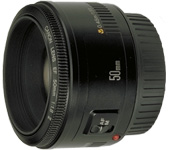
\includegraphics[width=0.4\textwidth]{canonef50mm-1}
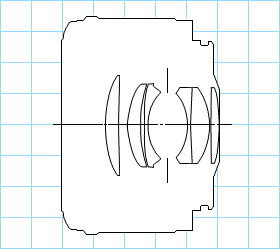
\includegraphics[width=0.4\textwidth]{canonef50mm-2}
}{fig:canonef50mm}{
	A fixed focal length Canon EF 50mm f/1.8 II camera objective.
	Left: the device, not attached to a camera.
	Right: block diagram of the lens construction, showing the six optical elements.
	Diagram by Canon Camera Museum.
}


The following relation applies for a thin lens or a system simplified as one, and an image in focus, as seen in figure \ref{fig:thinlens}:

\begin{equation}
	\frac{1}{a} + \frac{1}{b} = \frac{1}{f} \label{eq:focal}
\end{equation}

\simplefig{h!}{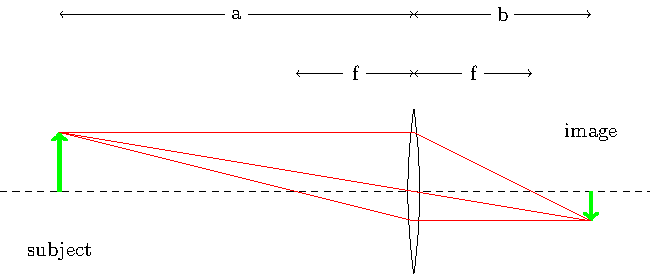
\includegraphics{lens}}{fig:thinlens}{
	thin lens sample: $a=6$, $b=3$, $f=2$. Actual subjects would be usually much further away; image depicts a macro setup for clarity.
}

where $f$ is the focal length of the lens, $a$ is the distance between the lens and the imaged subject, and $b$ is the distance between the lens and the camera's image sensor. Figure \ref{fig:thinlens} shows an example where the lens magnifies the subject at a factor of less than one, making it smaller on the camera film.
% hox, optical axis
% TODO: fig:focal

%The focal length has a direct influence to field of view, as given in figure TODO. Longer focal length (long-focus lens, often referred to as telephoto lens) results to a more zoomed in picture, as opposed to a wide-angle lens. 

% Aperture.

\emph{Aperture} refers to the minimum size of the hole where light effectively goes through; the hole itself is called \emph{aperture stop} and is located in the middle of the objective.
if it is not infinitesimally small, as in any practical case, there will be some area of the scene that is imaged as sharp and others in front and behind of this area will be blurred.
This effect is called \emph{depth of field (DOF)}.
In artistic photos, it can be preferred to have a small subject in focus to separate it from the background by blurring the background.
In 3D reconstruction, exactly the opposite is preferred: everything should be in focus.
%This might require a really small aperture, and consequently really bright lights, in a reconstruction rig where the distance to the subject is relatively short.

As the blur happens gradually, a \emph{circle of confusion} (CoC) is often used as a definition of unsharp areas of images.
A point outside the focal plane shows up on the image sensor as a circle (for circular apertures); when this circle is significantly larger than the pixel size on the sensor, the point is perceived as blurred.

Depth of field is defined as difference between the shortest and farthest object distances that still generate an acceptable CoC, found geometrically.
When $f$ is the focal length, $F$ the aperture f number, $s$ the distance to the subject, and $c$ the maximum acceptable CoC, the depth of field $D$ is given by (\cite{greenleaf1950photographic}):

\begin{equation} \label{eq:dof}
	D = \frac{2 s f^2 F c (s - f)} {f^4 - F^2 c^2 (s - f)^2}
\end{equation}

\simplegfx{h}{\textwidth}{dofcoc}{
	Exaggerated illustration of depth of field and circle of confusion with a thin lens, seen from the side (not drawn to scale).
	Sensor is at the green line, and the middle of the cross represents the lens.
	Subjects at distance $s$ project perfectly at the sensor.
	Distances between $Z$ and $Z'$ project to a circle smaller or equal to $c$.
	It can be easily seen that for subjects at longer distances, the depth of field increases.
}


In figure \ref{fig:dofcoc}, $Z' - Z = D$, the maximum and minimum acceptable distances near the subject.
Sufficient depth of field is important to consider in near-field 3D scans with small subjects, which translates to a small aperture, and consequently, really bright lights.
The subject should fill whole image frame to use the pixel density effectively.
Increasing the distance to the subject would increase depth of field, but enlarging the subject in the frame again would need a longer lens, which decreases depth of field.

Size of the CoC depends on the resolution power of the viewer; when a photograph is looked with the eye, the print size of the image determines the circle.
A standard-considered formula in photography determines the maximum acceptable CoC by dividing the image size by 1500, originating from human eye and looking distance.
For the standard ``full-frame'' 35 mm film size with an image size of 36 x 24 mm (about 43 mm diagonal), the CoC becomes $c = 43 \text{mm} / 1500 \approx 0.03 \text{mm}$.
In reality, an intuitive way to determine the disk size is the size of a single pixel in a digital sensor;
the disk should not span too many pixels, so that accurate detail would be resolvable from the digital image.

For a normal 50 mm lens with the subject at a distance of 1 m, an aperture of f/11 and a circle of confusion of 0.03 mm, the formula \ref{eq:dof} gives $D \approx 25 \text{cm}$. % , having the subject approximately in the middle of the acceptable range.

% diffraction

\emph{Diffraction} is an effect that happens for too \emph{small} apertures.
When light rays diverge on a small aperture, their different distances traveled make the waves interfere each other and produce a two-dimensional diffraction pattern, called an \emph{airy disk}.
The disk blurs the image in a similar fashion as an object that is out of focus.
Size of the airy disk is relative to the size of the aperture.
Thus, the aperture size must be set to a balance between the unwanted effects of DOF and diffraction.
% d/2 = 1.22 lambda N http://en.wikipedia.org/wiki/Diffraction-limited_system

% rayleigh limit?

All practical optical systems introduce some non-linear \emph{radial} and \emph{tangential distortion} (depicted in fig. \ref{fig:distortions}) that affect the accuracy of the ideal pinhole model.
Common distortions are the purely radial so-called \emph{barrel} and \emph{pincushion} distortions, where the lens magnification is a nonlinear function of image ray distance from the center of the lens. \cite{brown1966decentering}
Other extreme distortions, such as the ``fisheye'' distortion present in extremely short focal length lenses, is usually not considered.
Most reconstruction software assume either undistorted images or use a simple distortion model, and give poor results with exotic lenses.

In addition to radial, tangential distortion is less significant, and it is often ignored.
Its cause is small misalignments in separate elements in a single optical system; lenses being offset from each other and not being parallel to the image plane. \cite{kingslake1989history}

Wilson \cite{wilson2004anton} discusses optical systems' relation to depth of field, focus and distortions.

\simplefig{h}{%
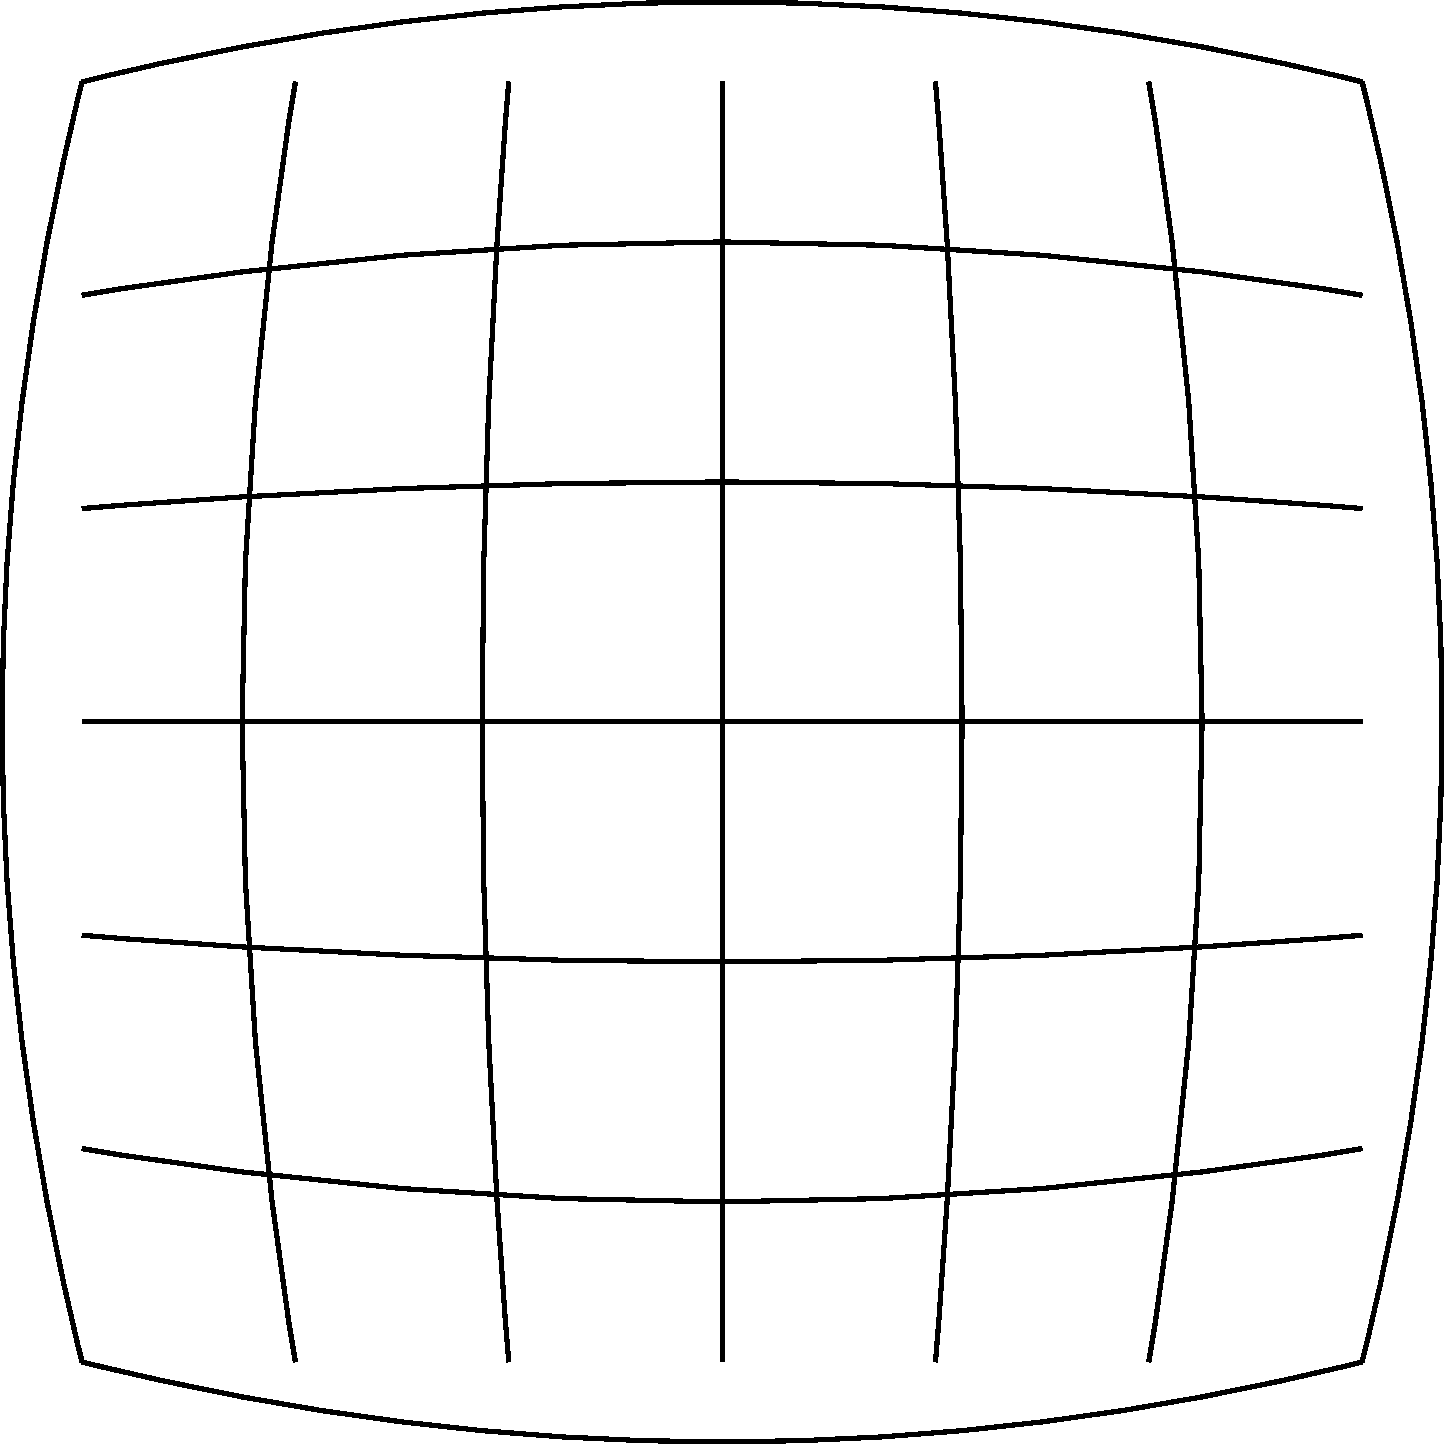
\includegraphics[width=0.2\textwidth]{barrel-distortion}
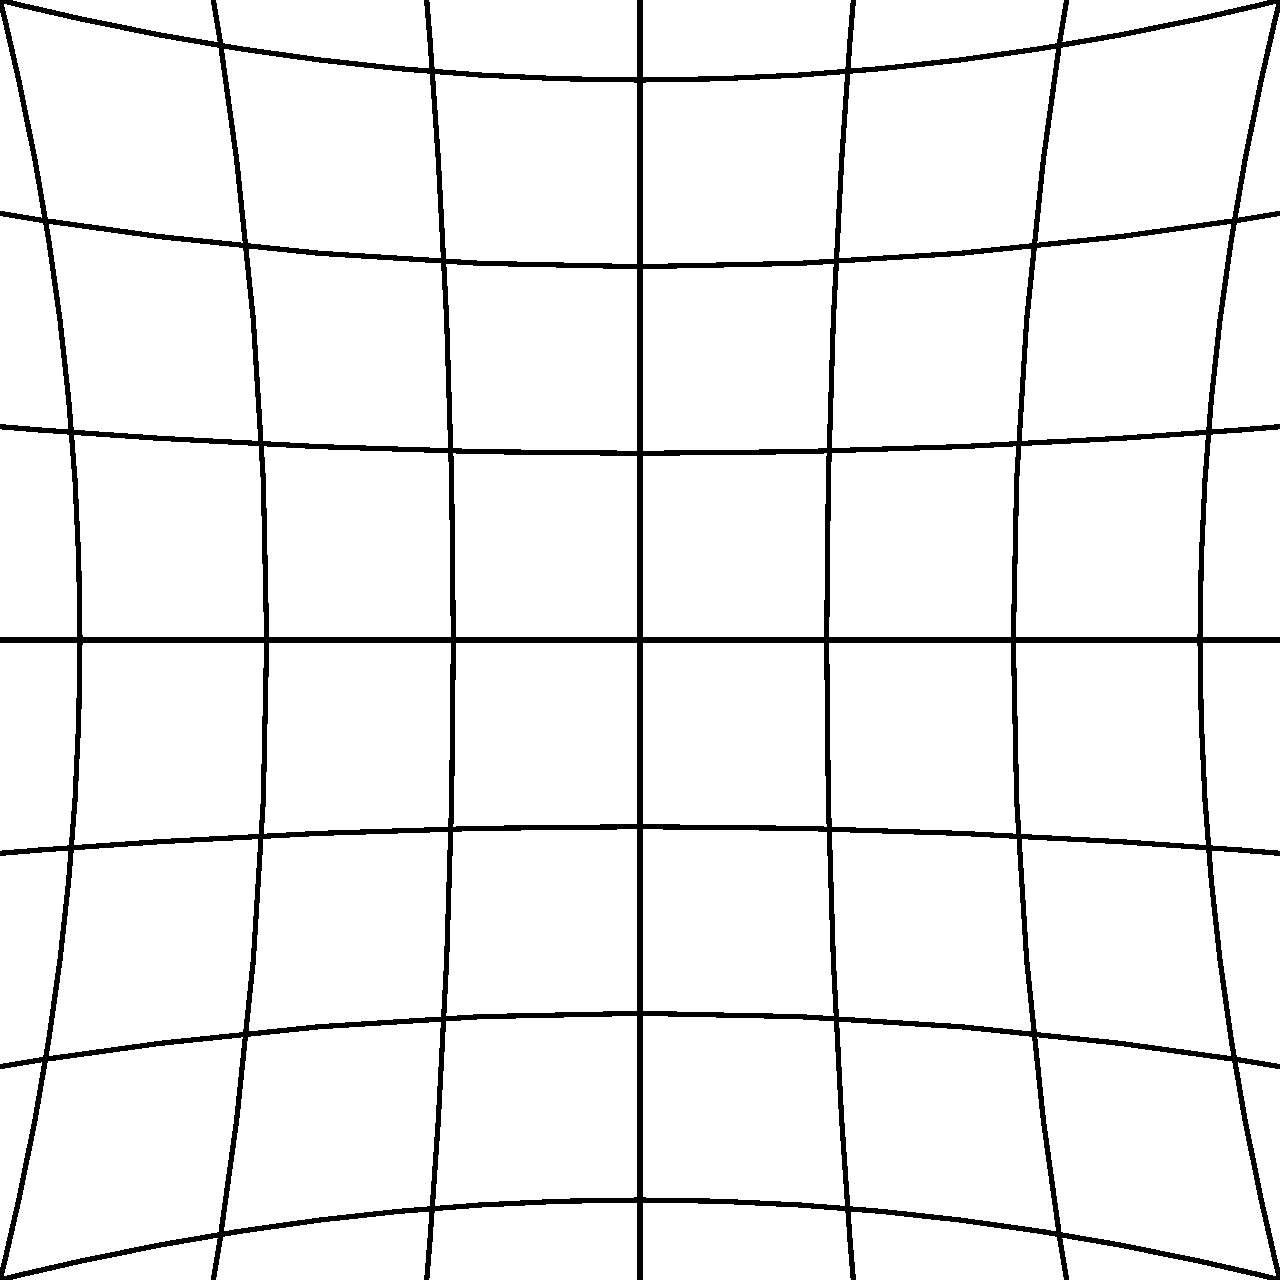
\includegraphics[width=0.2\textwidth]{pincushion-distortion}
}{fig:distortions}{
	Barrel (left) and pincushion distortions that would show up in an image of a grid of straight lines.
	For a lens with no distortion, the lines would not be curved.
}

Distortion should be corrected in software, as the following stereo algorithms assume that the images are free of nonlinear errors, i.e. straight lines in the world should remain straight in 2D images after the projective transformation.
%In particular, image rectification (discussed later in \ref{sec:rectification} won't work if this straightness does not remain; the assumption that similar features should be found on horizontal lines wouldn't hold on distorted images. \cite{hartley03multiview} 

The radial correction proposed first by Brown \cite{brown1966decentering} and used by e.g. the OpenCV library \cite{opencv} to create a new image of the original pixel values at new positions is

\begin{align} \label{equ:radialdist} \begin{split}
	x_{corr} &= x(1 + k_1 r^2 + k_2 r^4 + k_3 r^6)\\
	y_{corr} &= y(1 + k_1 r^2 + k_2 r^4 + k_3 r^6)
\end{split} \end{align}

% (XXX some software does this in a different way (inverse of this, maybe?)

Trucco and Verri \cite{trucco1998introductory} use only the two first coefficients.
For tangential distortion, the correction has the following form:

\begin{align} \label{equ:tangdist} \begin{split}
x_{corr} &= x + (2 p_1 x y + p_2 (r^2 + 2 x^2))\\
y_{corr} &= y + (2 p_2 x y + p_1 (r^2 + 2 y^2))
\end{split} \end{align}

In eq. \ref{equ:radialdist} and \ref{equ:tangdist}, $x$ and $y$ are the original coordinates in the distorted image, $x_{corr}$ and $y_{corr}$ are the corrected ones, $k_1$, $k_2$, $k_3$, $p_1$ and $p_2$ are coefficients specific to the distortion, and $r$ equals to the distance to image center where the optical axis hits, located at $(x_c,~y_c)$:

\begin{equation}
r = \sqrt{(x - x_c)^2 + (y - y_c)^2}
\end{equation}


The image size is often normalized such that the coordinates $x$ and $y$ range from $-1$ to $1$, making the distortion parameters universal for all image resolutions.
A barrel distortion with parameters $k_a = 0.04$ and $k_b = 0.02$ is shown in fig. \ref{raddist}.
% TODO: only first and also ka and kb for comparison

\simplegfx{h}{\textwidth}{raddist}{
	Barrel-type radial distortion with different parameters.
	Lines point from destination image pixels to locations to sample from in original image.
	Left: $k_a = 0.16$, middle: $k_b = 0.08$, right: $k_a = -0.04, k_b = -0.04$.
}

Because digital images consist of a discrete pixel array, the pixel coordinates given by the undistortion do not necessarily lie on exact pixel positions;
the sampling should then interpolate between neighboring pixels, instead of taking the nearest color.

%Perspective distortion something something viewer location.
%Normal TV is usually watched at the distance of twice the screen diagonal.
%At this location, the scene looks normal when taken with a normal lens.
%A wide-angle scene then looks normal when viewed at a nearer distance. \cite{wilson2004anton}

% 14:01:55 <naavis> Kai sillä yritetään emuloida sitä, että katsojan paikalta se leffan kuvakenttä vastais sitä että valkokankaan tilalla on ikkuna.

% }}} optics

\subsubsection{Image sensors} \label{sec:sensors} % {{{

% intro: film vs sensor

Historically, photographs were saved on a photosensitive film.
With digital cameras, a rectangular electrical \emph{sensor} replaces the film.
The sensor consists of a uniformly spaced grid of small pixel sensors built as an integrated circuit package.
A \emph{pixel}, or picture element, represents a tiny dot on a film; when combined, the dots form a larger picture.

% digital pics

Digital pictures on a computer are represented as rectangular arrays of numbers, or \emph{raster images}.
Each number describes the intensity of a single pixel on a specific location.
For a single intensity value per pixel, a grayscale picture would be obtained.
Color pictures are described with more intensity channels than one, in e.g. RGB space, the way that most parts of a computer use for describing colors.
A single RGB color encodes the intensities of red, green and blue separately.

% sensors

The rectangular image sensor senses the amount of light hitting each pixel and encodes it to an electrical signal.
The signal is digitized to a brightness value and the camera saves all the pixels to a file in mass storage.
There are two major sensor types: CMOS (Complementary Metal-Oxide Semiconductor) and CCD (Charge-coupled Device).
CMOS is the type used in most still cameras because of its lower price.

%It has some technical disadvantages, considering movie recording.
CCD captures a whole image frame at once (``global shutter''), while CMOS reads the sensor a single row at a time, resulting in an effect called ``rolling shutter'' \cite{todo:cmos}.
CCD has other issues, such as bleeding a strong light source to surrounding pixels and interlacing, i.e.~alternating in reading only odd and only even rows in consecutive frames.

% noise

As all electronic circuits, also image sensors are subject to signal noise.
Each pixel receives an additional random signal level that shows up as additive brightness, noticed usually only in low light conditions or black areas.
Noise increases with sensor's signal gain, or ``exposure sensitivity'' described using the ISO system (``film speed'').
A more sensitive sensor needs less light for a bright-looking image, because the signal is amplified more before digitization.
This amplification also amplifies the original signal noise, which is why the gain level should be kept as small as possible and the amount of light entering the sensor as large as possible.
This leads to using bright lights in the imaged scene or a longer exposure time.
Longer exposure time influences more motion blur, though.

% sensor movement

Some cameras use image stabilization by moving the sensor, as opposed to moving the optical elements inside the lens.
In any case, image stabilization should be turned off for reconstruction because it affects the calibration of image formation: if any element in the image acquisition path moves, calibration parameters also change.
The sensor also moves when a camera uses a sensor cleaning mechanism with ultrasonic vibration motor on the sensor.

% colors

A single pixel sensor acquires all light hitting it, independent of the wavelength.
Two principal methods to retrieve the red, green and blue color bands for each pixel are used in color cameras, one being cheaper and thus more common.
The most common method is to interleave red, green and blue in a single sensor by filtering the wavelength that can enter a pixel with a colored film over the sensor, with a special repeating pattern called \emph{color filter array}.
The missing values for other colors bands are interpolated from surrounding pixels.
The most popular interleaving pattern is the Bayer filter, illustrated in figure \ref{fig:bayerpattern}.
Other arrangements of red, green and blue are also used, some incorporate other colors, such as cyan, yellow, green, and magenta.

Another way is to retrieve the three channels with three different sensors, one for each wavelength band, and to guide the light to them with prisms and filters; being more expensive than a single sensor, this method is used in some high-end cameras only.

\simplefig{h}{\bayer{0.6}}{fig:bayerpattern}{
	A small partly drawn subset of the repeating Bayer pattern.
	Each square is a single pixel; the grey area represents the image sensor.
	The gap between pixels is nonzero.
}

% ???

Physical pixels cover less than the full area of a sensor, as there are gaps between them;
microlenses between the pixel sites direct the light hitting the gaps to the neighboring pixels, with varying color performance.
Because of the discrete nature of the pixel array, some cameras employ an analog low-pass filter in front of the sensor to hide high-frequency information that would show up as aliasing.

% support electronics

Near the pixel sensors and their amplifiers is digital logic for reading out the data and passing it through to an image processor.
Quality of this support electronics affects some properties, most important of which are analog-digital converter noise and dynamic range, and speed that the image is read out from the sensor.
A so-called raw image file can be saved with more expensive cameras contains the raw sensor data with very little processing done;
when a raw file is not used, the camera processes the image with device-specific correction filters and applies e.g.~white balance correction, and finally saves the image as a standard image file such as JPEG.
Clock speed of the conversion circuits with the main processor speed ultimately determine the maximum burst imaging speed.
For example, for the Canon flagship camera EOS-1D X, a continuous shooting speed of 14 frames per second is advertised.
With its resolution of 5184 by 3456 pixels and 14-bit processing, an estimate for the bit rate from the sensor is

\begin{equation} \label{eq:eos1dspeed}
5184 \times 3456 \times 14 \times 14 \approx 3,5\text{ Gbit/s}
\end{equation}

by average, or 0,4 gigabytes per second, requiring also high speed from the processor and mass storage.
In reality, a number of other complicated factors also have a small effect.

% }}} image sensors

\subsubsection{Shutter} % {{{

% shutter, why needed

A static scene is imaged by exposing the sensor to the light passing the optics for a short time, keeping the camera and subject steady.
Electrical sensors can be cleared to black rather quickly.
Still, good quality cameras use even faster mechanical shutters for photographs.
Because of the rolling shutter effect of a CMOS sensor, it is better to do the reset and readout phases when the sensor is not exposed to light.

% mechanical stuff

\simplegfx{h!}{0.8\textwidth}{focalplaneshutter}{
	Focal plane shutter has two moving curtains to cover the sensor, opening it momentarily so that each pixel receives light for the same amount of time.
	From left to right: initially, the sensor is blocked.
	Once the first (red) curtain moves away, the sensor is exposed to light.
	A second curtain (blue) stops the light from entering again.
	The shutter resets by moving back to the position in the top (not shown).
	Modern shutters actually have folding metal pieces to save space, but the effect is the same.
}

\simplegfx{h!}{0.8\textwidth}{focalplanerolling}{
	Rolling shutter effect in a focal plane shutter happens when the exposure time is really short.
	The shutters have to move at the same time, exposing only a part of the sensor at a time.
	Fast movement during the exposure leads to artifacts and a short flash light would illuminate only a part of the sensor.
}


A \emph{shutter} is a mechanical device that blocks light to the sensor and can be moved quickly out of the way and back.
There are several types of mechanical constructions for shutters, depending on the application.
Some compact cameras have a small \emph{leaf shutter} in the lens center that can be moved fast.
A \emph{focal plane shutter}, used in most system cameras, is installed in front of the sensor.
It consists of two curtains that move to the same direction; one moves out of the way of the sensor to let light pass to it, and another moves to cover it back again when the exposure time has elapsed.
Figure \ref{fig:focalplaneshutter} illustrates a planar shutter (in reality, the curtains are black and not complete planes).

A \emph{rolling shutter} effect is produced with very high shutter speeds, where the limit of curtain movement speed prohibits fully opened shutter and the closing curtain starts to move before the first has stopped, exposing only a narrow band of the sensor at a time.
Fast mechanical shutter movement is depicted in figure \ref{fig:focalplanerolling}.

%Result of shooting a moving object with rolling shutter is depicted in figure \ref{rollingeffect}.
When an object is moving to the same direction as the narrow shutter slit, i.e. vertically, it appears smeared;
when the movement is horizontal, different parts of the object appear to bend.

%\simplegfx{h!}{0.8\textwidth}{rollingeffect}{
%	Rolling shutter imaging a spinning disk.
%	At each point in time, the slit captures only part of the subject.
%	When the object moves, the subject appears distorted.
%	Image by Wikipedia user Cmglee, licensed under CC BY-SA.
%}

A digital CMOS exposure and ``electrical shutter'' works like this too; the sensor is reset and read row by row sequentially; this produces a strong rolling shutter effect especially in video cameras when the subject is moving fast relative to the camera.

A CCD camera would not need a mechanical shutter, because the full image is read out at once.
Most still cameras have also a movie mode that holds the mechanical shutter open all the time, using the electrical shutter.

The mechanical shutter can last only a finite amount of actuations (50 000-200 000 for a common system camera) as it wears out gradually.

% other

When the camera or the imaged subject moves while exposing the full frame, an object gets smeared along the movement on the image, an effect known as ``motion blur'': the image gets blurred where motion happens.

Video film cameras that capture each frame to a separate part of film used a spinning wheel with a transparent window, called rotary disc shutter. \cite{wilson2004anton}
This rotates at a precise speed synchronized to the frame rate, displaying a for a consistent duration for each frame.
The size of the window constitutes to the amount of light and motion blur.
Video is more discussed in the section \ref{sec:video}.

When taking a picture, the camera does not instantly start to expose the image.
Each camera has a specific \emph{shutter lag} that is the time that elapses between when the shutter button is pressed and when the shutter moves out of the way.
Some sources include in this term also the time for the camera to focus the lens and measure sensitivity settings which can be a significantly longer time.

Shutter speed has small variations over time when the camera ages and some parts wear out.
Some difference also exists among same camera model from mechanical variations and software processing.
When using a flash unit instead of continuous light, the short duration of the bright flash of light must happen when all the cameras have opened, but not yet closed, their shutters.

%Shutter lag (auto exposure/focus even in manual mode maybe?)

% }}} shutter

\subsubsection{Lighting} % {{{

In addition to multiple cameras at different locations and poses to encode a subject's geometry, a uniform and soft lighting is also required for consistent color reproduction and to minimize bright reflection difficulties in the texture.
A large variety of different studio lights are available in the market for different lighting situations, emitting either continuous light or short bright flashes.

% XXX pic of brightness constancy: same object from two views, patch windows
Because most reconstruction methods fundamentally assume a relatively diffuse lighting, a property called \emph{brightness constancy} (i.e.\ the brightness and color of a surface looks the same from all viewing directions), they perform poorly when a light shines off a surface so that its specular highlight is at a different geometric location in different images.

%\simplegfx{h!}{0.7\textwidth}{brdfdiagram}
%{BRDF of a surface is a function of surface normal $n$, light direction $\omega_i$ and viewing direction $\omega_o$.}

Surfaces can be modeled as \emph{diffuse} and \emph{specular} components that are functions of light direction, viewing direction and spatial location on the surface.
Surface reflection models are described with a bidirectional reflectance distribution function, or BRDF. \cite{nicodemus1965dirreflectanceetc}

A distribution model of the surface's global or local microgeometry specifies how much light reflects in different surfaces. \cite{nayar1991surface} % XXX 1991 or -89? TODO fig 22 from the paper
Diffuse means a material that reflects light uniformly to all directions, depending only on the angle between the surface normal and light location, whereas more specular surfaces are composed of a different microstructure that reflects light in a more mirror-like way and the surface brightness depends on where it is looked from.
%Diffuse surfaces are called matte or Lambertian; they follow Lambert's cosine law (equation \ref{eq:lambertcosine} often used in computer graphics), a lighting model, shown in figure \ref{fig:lambertcosine}. \cite{lamberttodo}
%A Lambertian surface's BRDF is constant among the viewing direction.
\emph{Specular highlight} or \emph{specular reflections} refer to a mirror reflection of the lamp on the imaged surface.
In figure \ref{fig:nayarbrdf}, different types of reflections seen by the camera are visualized as light intensities of different colors.
Ideally, the camera would only record the diffuse reflection that represents the surface color;
the specular components are unwanted artifacts.
Polarized filters can be used in front of the lights and in the camera lenses to filter out most of the specular lighting.
%Surfaces modeled in computer graphics are often relighted with functions of surface normal and light and view directions, given as unit vectors, as in figure \ref{fig:brdfdiagram}.

%\begin{equation} \label{eq:lambertcosine}
%	I_D = L \dot N I_L = |N| |L| \cos \alpha = \alpha
%\end{equation}

\simplegfx{h!}{0.7\textwidth}{nayarbrdf}{
	Polar plots of three reflection components as functions of the viewing angle, as suggested in \cite{nayar1991surface}, showing the brightness seen from different angles from the surface normal.
	In a reconstruction subject, the bright specular spike and lobe reflections should be minimized, and only the diffuse color is wanted.
	Image by Nayar \cite{nayar1991surface}.
}

Commonly used terms such as ``soft'' and ``hard'' lighting refer to the size and power of light sources: bright spotlights are hard, and larger and relatively less bright lamps are soft.
Softness can be added by increasing the light's area while holding its power constant, such as reflecting a light off a large surface or adding a white cloth between it and the imaged subject.
%Effects of a soft versus hard light are illustrated in figure \ref{fig:lighthardness}.

Powerful electronic flash units use usually a gas-filled tube that is excited with high voltage to produce a short, bright burst of light for some milliseconds.
Flashes are good for portrait photographers because the subject sees the bright light only for a short moment; thus, the light does not annoy the subject.
Short bursts of light in an otherwise dark environment are also good for stopping motion and synchronizing multiple cameras, as only a short time is effectively exposed to light.

%dark contact lenses if available (remedy)

%bodies' own flashes maybe not uniform enough; too many flashes i guess

%softbox or umbrella

%Polarization filter

% }}} light sources

\subsubsection{Image download} % {{{

% data path intro

The image information travels from the subject through the optics to the image sensor's surface, via an analog/digital converter, the camera's processor(s) and finally to a memory card or straight to a computer's storage via a wired or wireless connection.
Many parts in this path contribute to the rate of which the images can be taken, usually measured in frames per second (FPS).

% fps

An average DSLR can achieve around five frames per second of full resolution footage, while more expensive models can reach over 10 FPS.
A digital still camera can often record video too, at a lower resolution and a higher FPS.

% XXX \ref{eq:eos1dspeed}

% files

The raw files saved by DSLR cameras are compressed in a proprietary lossless format and contain also metadata about certain camera settings.
%Lossless compression maintains image quality and reduces file size depending on the complexity of the frame.
%Some manufacturers encode the brightness values through a lookup table, and it's common to use a compression scheme known from standard file compressions, or a specific lossless image compression.

Raw video consumes too much data to be feasible to use normally.
Video files are almost always saved in a lossy video format, the H.264 format being common for modern cameras.
Compression introduces loss of detail and artifacts typical to each algorithm, often visible as blocks or blurring.
Common bitrate for a full-HD (1920 by 1080 pixels) 24 FPS video is about 5 MB/s.
Reconstruction from frames extracted from a compressed video may not be as good as from separately saved stills.
Some expensive cameras can record raw video, and others can be tricked to that.
Canon DSLRs can be tricked to dump the raw stream to a memory card, but only some models support the faster CF memory cards that can keep up with the amount of data with useful resolution.

% storage

In consumer devices, files are stored to a removable memory card.
Industial devices transfer the images directly to a PC via a wire.
Memory cards used by consumer grade cameras (Compact Flash (CF), Secure Digital (SD)) can support speeds up to 125 MB/s and capacities in tens of gigabytes.
The speed of USB 2.0 high-speed specification is 480 Mbit/s; bus protocol's overhead limits effective data throughput to around 80 \%.
Machine vision cameras use a higher speed connection, such as the newer USB 3.0, IEEE 1394 (FireWire), gigabit Ethernet or Camera Link to achieve realtime lossless transfer of high-resolution images.
For example, the 1 Gbit/s Ethernet connection can transfer a raw 12-bit full-hd stream at

\begin{equation} \label{eq:gigabit-transfer}
	\frac{1 \text{Gbit}/s}{1920 * 1080 \text{ px} * 12 \text{bit}/\text{px}} \approx 43 \frac{1}{s}
\end{equation}

where Gbit is $1024^3$ bits.

%http://majid.info/blog/is-the-nikon-d70-nef-raw-format-truly-lossless/

% }}} image download

\subsection{Video} \label{sec:video} % {{{

%Hox ALL-I (intra) vs. IPB (intra-predict-bidirpredict)

% intro, connection to reconstruction

\emph{Video} is ordered electronic pictures displayed one after another.
Humans perceive motion when a previously seen object is seen again in a nearby location.
Current digital video technology encodes motion pictures as in films, in a sequence of still images, recorded and displayed at a constant rate.
Three dimensional motion is generally no different: it is encoded as discrete poses in sequence.
In order to do motion capture in stereo vision, video material from two or more of cameras is used to initially capture a sequence of still photos.

To reconstruct the frames in 3D, each set of frames encoded by the cameras should be \emph{synchronized}, i.e.\ shot at the same time, because the reconstruction assumes a static subject.

% }}}

\subsubsection{Sequence of frames} % {{{ or: video is frames

% how/when frames are captured

When scanning a scene continuously, a camera shoots frames using the same principles as in photos, but does it in sequence, at a speed that is called \emph{frame rate}.
For each frame, the shutter is open for a duration of \emph{exposure time} or interchangeably \emph{shutter speed}.
In \emph{interlaced video}, two frames make up a whole picture that covers all pixels.
Interlacing alternates between odd and even lines to increase update rate, and was invented for cathode ray tube displays to reduce apparent flicker.
The alternation results in tearing artifacts when imaging horizontally moving subjects (shown in figure \ref{fig:interlace}).
Many CCD video cameras still produce interlaced stream, because it is cheaper to manufacture due to fewer pixels.
Video that contains full frames only is called \emph{progressive}.

\simplegfx{h!}{0.7\textwidth}{interlace}{
	A cropped area of interlaced scanning.
	From left to right: even lines only, odd lines only and full picture combined.
	Top: stationary square.
	Bottom: a moving square, showing tearing if the frames would be combined.
}

% on fps

Consumer video cameras, video-capable pocket cameras and DSLRs typically offer a few choices of frame rate. Traditionally, the movie industry has used 24 FPS; 25 and 30 are common alternatives used in TV broadcast, some cameras being capable to twice the speed at a lower resolution.
Actual FPS is slowed down from the advertised by a factor of 1.001 because of historical reasons in monochrome and color TV backwards compatibilities.
30 and 24 FPS refer to approximately 29.970 and 23.976 FPS, respectively.

Externally triggered cameras can be configured to record at any arbitrary rate and exposure, as long as it's in the limits of the camera speed capabilities.
Synchronized machine vision cameras do not record video on their own, but instead just monitor to a synchronization signal and output frames on its rate, that frame grabbers on a computer read and store.

% dslr sucks

DSLR video modes use almost the sensor's full size but skip some of its lines when recording video, resulting in the same field of view as still images but suffering from significant aliasing patterns with certain subjects with high frequency information.
Additionally, pixels in the video frames do not represent physical pixels anymore, posing awkwardness in camera calibration.
Line skipping is depicted in figure \ref{fig:lineskipping2}.
The color filter array makes the problem even worse for small-detailed features of high color detail.

\simplegfx{h!}{0.5\textwidth}{lineskipping2}{
	Line skipping in a DSLR camera in video mode.
	Left shows a part of the full sensor and its bayer pattern; on the right, only every third line is captured.
}

% }}}

\subsubsection{Frame rate and shutter speed} % {{{

\simplefig{h}{
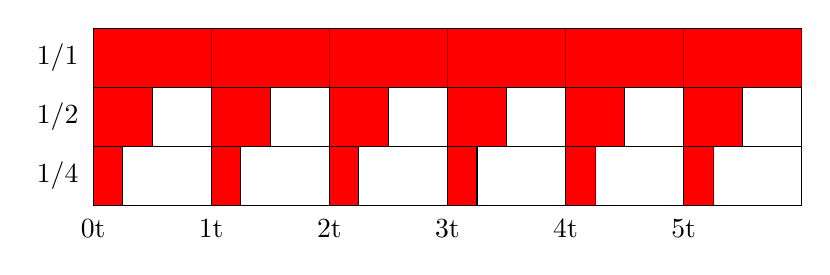
\begin{tikzpicture}[scale=1.5]
	\def\nframes{5}
	\draw (0,0) rectangle ++(6,-1.5);
	\draw (0,-0.5) -- ++(6,0);
	\draw (0,-1) -- ++(6,0);
	\foreach \x in {0,...,\nframes} {
		% time ticks
		\node at (\x*1, -1.7) {{\x}t};

		% exposure blocks
		\draw [fill=red] (\x*1, 0) rectangle ++(1.0, -0.5);
		\draw [fill=red] (\x*1, -0.5) rectangle ++(0.5, -0.5);
		\draw [fill=red] (\x*1, -1) rectangle ++(0.25, -0.5);
	}
	\node at (-0.3, -0.25) {1/1};
	\node at (-0.3, -0.75) {1/2};
	\node at (-0.3, -1.25) {1/4};
\end{tikzpicture}
}{fig:shutterspeed}{
	Varying shutter speed compared to constant frame rate, FPS is $1 / t$.
	Red rectangles illustrate exposure time, i.e.\ open shutter.
	For an always open shutter, the camera records everything.
	A ratio of 1/2 is a ``normal'' rate.
	1/4 results in slightly less motion blur.
}

A higher frame rate results in more accurate representation of motion as a whole, and a faster shutter speed helps to reduce motion blur in individual frames.
Ideal exposure time would be infinitesimally short; practically, the amount of available light restricts the time, even though a camera would be faster.
Similarly, what happens when the shutter is closed is not recorded; ideal frame rate would be faster than any period of motion in the scene.
For motion tracking based on frame differences, a long enough time should be passed for reliable motion direction, though.
Normally, if playback happens at a different rate from the recording, motion is interpolated between different frames or the last appeared frame is used.

In contrary, in motion picture industry, the shutter is kept open deliberately so long that fast motion is blurred, because it is considered aesthetically pleasing to human eye;
even though the motion is blurred, more temporal information about the scene movement is encoded per frame than when exposing infinitesimally short frames, at the expense of spatial resolution.
A common shutter speed relates to frame rate such that a frame is exposed half of the time between frames.
\cite{wilson2004anton}
Good cameras allow to change the frame rate and shutter speed independently.

Film cameras and some professional video cameras use a rotary disc shutter that has an opaque 180 degree sector.
Having half the exposure time of frame rate is sometimes called ``180 degree shutter''.
While the light is blocked, film is mechanically advanced to the next frame.
Digital video analogously downloads data from the image sensor and clears it during this time.

For unsynchronized videos that shoot frames at different points in time, morphing techniques have been developed to analyze motion between frames and to interpolate intelligently.

%Motion blur encodes more information about object travel but gets less precise by time.
%slowmovideo \cite{eugster2011slowmovideo}

% }}}

\subsubsection{Multi-camera synchronization} % {{{

%Time offset / drift / jitter / lockstep

Synchronized recording of multiple view video is more complicated than shooting still photos simultaneously.
The cameras should be clocked together to hold their shutters open at the same time during each frame.
An assumption of stereo vision is that the images encode a static scene, i.e. geometrically same objects, which would not hold otherwise.
This can be compensated to some degree with optical flow if hard syncing is not possible. \cite{bradley2009synchronization}

Synchronization issues can be divided roughly in three sources of error, assuming N cameras each having its own video file with same frame rate: \emph{offset}, \emph{drift} and \emph{jitter}.
With the same frame rate, the frames can be indexed with numbers starting from 0.
Times when the frames taken relative to a global clock is noted as $t_{Ci}$, where $C$ is a camera identifier and $i$ is the increasing frame index.
% TODO something on the errors modulo frame length

\emph{Offset} is the time difference of two streams: for an ideal camera $A$ at each frame $t_{Ai}$ for $i$, and an offset camera $B$ at $t_{Bi}$, a constant error $e$ is added:

\begin{equation} \label{eq:timeoffset}
	t_{Bi} = t_{Ai} + e
\end{equation}

Drift is a property of one a camera that advertises to record at some speed and actually works at some other speed. Similarly, for cameras $A$ and $B$, constant $d$:

\begin{equation} \label{eq:timedrift}
	t_{Bi} = t_{Ai} + d i
\end{equation}

Jitter is the random difference $j(i)$ between frames for a same camera:

\begin{equation} \label{eq:timejitter}
	t_{Bi} = t_{Ai} + j(i)
\end{equation}

For an actual video camera, drift and jitter are negligible; offset originates from starting the recording at a different time and from camera's internal processing before the recording actually starts.
If the cameras take pictures only when instructed, such as machine vision cameras, a common clock generator becomes another source of errors.
Many consumer cameras support a live preview feed when connected to a computer; the feeds can be useful for previewing but jitter becomes too significant because cameras are not designed with this in mind.
If the offset between two cameras is not an exact multiple of the frame speed, they effectively cannot have any frames that would display exactly the same scene.

Frame accurate offset sync with clapperboards works by matching the clap sound to visual cues in the video, a method well known in film production.
Cameras that record audio to the same video file do not need visual cues and can be synced together by matching just the sound streams.
%This is the method used in making movies when editing a final version with multiple cameras used.
Unsynchronized shooting still leaves at most half a frame lag between the camera sequences; this is illustrated in figure \ref{fig:syncproblems}.

Professional video cameras can be synced to a single clock generator, so that they all operate on the same frequency (i.e. no drift) and phase (i.e. no offset), called \emph{genlocking} or \emph{generator locking}.
Similar method is used when shooting with machine vision cameras that have external trigger input.
Synchronizable camcorders are very expensive, and consumer-grade hardware usually lacks all possibilities for proper sync.

%\begin{verbatim}
%Drift
%
%normal   |   |   |   |   |   |   |
%drifting |    |    |    |    |    |
%         0t  1t  2t  3t  4t  5t  6t time -->
%
%
%Jitter
%
%normal   |   |   |   |   |   |   |
%jitterin |    |  |   | |      |    |
%         0t  1t  2t  3t  4t  5t  6t time -->
%\end{verbatim}

%Often used techniques are starting flash (does not need an audio track) [REF], clapperboard [REF], strobe sync'd to fps, genlock.

\simplefig{h}{
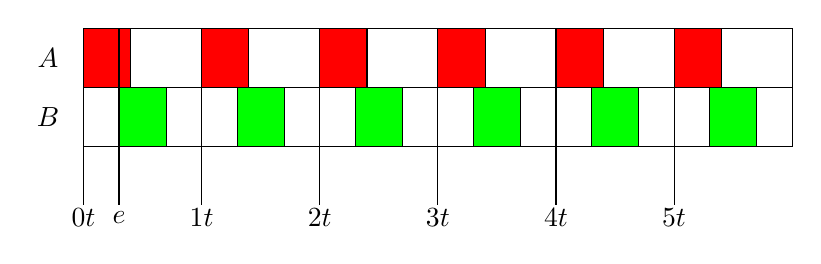
\begin{tikzpicture}[scale=1.5]
	\draw (0,0) rectangle ++(6,-0.5);
	\draw (0,-0.5) rectangle ++(6,-0.5);
	\foreach \x in {0,...,5} {
		\draw (\x*1, 0) -- (\x*1, -1.5);
		\node at (\x*1, -1.6) {${\x}t$};

		\draw [fill=red] (\x*1, 0) rectangle ++(0.4, -0.5);
		\draw [fill=green] (\x*1+0.3, -0.5) rectangle ++(0.4, -0.5);
	}
	\draw (0.3, 0) -- (0.3, -1.5);
	\node at (0.3, -1.6) {$e$};
	\node at (-0.3, -0.25) {$A$};
	\node at (-0.3, -0.75) {$B$};
	% P, Z
\end{tikzpicture}
}{fig:syncproblems}
{Video phase difference, i.e.~offset.
Red rectangles illustrate exposure times of camera $A$, green rectangles the same for camera $B$.
Frame period is $t$, and the cameras have a constant exposure time offset of an arbitrary $e$.}

% }}}

\subsection{Digital camera types} \label{sec:cameratypes} % {{{

% intro on camera types, wanted options left in implementation

This section quickly reviews the most common types of digital cameras available.
More in-depth survey on properties important in reconstruction are given in section \ref{sec:cameracomparison}.
%
%Good properties are image quality, configurability, ease of use and low price.
%Technical qualities usually get better with price.
%For a multi-camera setup with a restricted budget, low price is one of the largest advantages.
%On the other hand, large amounts of manual work should be avoided if possible; cheaper devices are usually more clumsy to use, as they lack manual controls.
%
% camera types introduced

\emph{Consumer cameras} have good availability, but they are targeted for artistic photographs and basic users.
They are divided roughly in two categories: \emph{compact (pocket, or point-and-shoot) cameras} and \emph{system cameras}.
The presence of a mirror divides system cameras in two: \emph{digital single-lens reflex cameras (DSLR)} and \emph{mirrorless interchangeable-lens cameras (MILC)}.
A MILC lacks a separate viewfinder and the reflex mirror, resulting in smaller size.
System cameras typically support an interchangeable lens and a number of auxiliary hardware, such as electronic flash units, remote shutter releases and power adapters to replace batteries.

\emph{Industrial cameras} for \emph{machine vision}, targeted for engineering applications, are more controllable and contain no unnecessary bulky parts, but are more expensive and may need proprietary control tools.
Their product cycle is typically longer and thus more reliable than in consumer electronics.
In industrial cameras, the different parts of the system are typically defined more accurately in terms of e.g.\ lens quality, sensor and pixel size, sensor noise, processing speed and communication protocol.

\emph{Camcorders}, video cameras with recording capabilities, also vary from consumer to professional grade devices.
Camcorders are not considered in this work because of their lower resolution relative to still cameras.

% some properties

Camera resolution, is declared in million pixels, or megapixels (Mpix).
Resolution and image size are related via pixel size that is the physical size of one photosite on the sensor.
Pixel size is described as the length of one side, and the pixels are typically square.
Newest consumer DSLRs can have a resolution of up to 20 megapixels.

% sensors

Typical sensor sizes for different camera types are as follows:

\begin{itemize}
	\item System cameras use a ``full-frame'' (36x24 mm) or APS-C (1.5-1.6x crop of full frame, i.e.~about 22x15 mm), resolution usually over 15 Mpix with pixel size at about 5 micrometres
	\item Compact cameras use a small sensor; sizes vary but are typically 1/2.3" (6.2x4.6 mm), resolution about 10 Mpix
	\item Smartphones use sizes between 1/3"-1/4" (less than 4.8x3.6 mm), resolution between 3 to 8 Mpix
	\item Sizes used by industrial machine vision cameras vary by application, in 5 to 10 mm range having resolutions from 0.5 to over 10 Mpix.
\end{itemize}

%sensor vibration to remove dust -> sensor position not very fixed \cite{rieke2009}. % TODO MEASURE!
%no image stabilizer in sensor or lens \cite{photogrammetry.doc}
%ring flash bending the lens assembly if attached to it \cite{rieke2009}.

% http://www.agisoft.ru/forum/index.php?topic=1411.60

% lenses, shutters

To benefit from the sensor resolution, the lens should have an equivalent or better \emph{resolving power} (i.e.\ \emph{contrast}), provided as a chart of \emph{modulation transfer function} (MTF).
A lens attenuates the frequencies of the optical patterns, such that at some point, tight line pairs are not resolved from each other.
Machine vision cameras and system cameras have by interchangeable lenses with often well specified MTFs, while cheaper compact cameras, phones and webcams are designed for a single lens that cannot be removed and has less defined MTF.
Compacts also accompany a zoom lens; zooms are more complex systems and therefore more expensive to reach a good image quality.
Calibration is also a problem with moving zoom elements that may not align to precisely same setting.
System cameras have a large selection of fixed focal length (``prime'') lenses.
The lack of zoom of a prime lens is preferable in a controlled environment, where the distance to the subject can be adjusted as necessary.
With DSLRs that have a moving mirror and a shutter, the mechanical vibration could move the zoom lens each time a little, changing the focal length.
Some compact cameras have a lightweight leaf shutter in the lens, and many use digital shutters.

%Lens sharpness is defined via their performance to high contrast, measured with modulation transfer function (MTF).
%Perceptual pixel count relates to lens contrast; a high pixel count sensor for a poor quality lens is only useful for observing the lens defects.

%Rieke-Zapp et al \cite{rieke2009evaluation} address several problems in camera calibration and imaging quality.

% storage

Storage size and speed and camera processing power in general follows camera price.
High-quality capture of short motions is aided by continuous burst mode that can achieve anything between 2 and over 10 frames per second, depending on camera model.
Professional-level DSLRs can handle over 10 continuous raw full frames per second, while entry-level DSLRs handle around five;
compact cameras are generally slower.
Machine vision cameras with resolutions comparable to DSLRs also exist, but at a significantly higher price.
Overall storage speed is determined by several factors between the sensor, the camera's processor and mass storage.
Reading the pictures to a computer can be done via USB or a memory card reader; the latter method is inconvenient as the card must be removed from the camera and placed to a reader manually.
Industrial cameras typically have temporary memory for only one frame that is read out immediately via a bus.
For video recording, this needs relatively large amounts of auxiliary hardware to save the raw frame feed.

% software support
Major consumer manufacturers provide a software development kit (SDK) for controlling their cameras remotely at some degree, and some support a common standard for file access.
For machine vision cameras, manufacturers provide their own software packages, in addition to sometimes specifying that the camera complies to a standard.
The standards specify data formats, image streaming and control methods.
Key standards for industrial cameras are:

\begin{itemize}
	\item Camera Link, partly proprietary (but significantly reverse-engineered) serial transfer protocol with special cable and connector types
	\item GigE vision, standard interface for video data over gigabit Ethernet connection; licensed so that writing open source software directly based on the standard is not officially possible
	\item IIDC/DCAM, Instrumentation \& Industrial Digital Camera or 1394-based Digital Camera Specification, data format standard used in IEEE 1394 (FireWire) cameras; an open specification
	\item USB3 Vision, a standard for the USB 3 bus
\end{itemize}

A standard-compliant industrial camera enables to use readily available software, reducing the need for in-house software and protecting from vendor lock-in.
Some of the largest manufacturers that offer standards-compliant cameras are Point Grey, Basler, Allied Vision, and Imaging Source.
%Coriander \cite{coriander} is a free user interface for controlling IIDC cameras.

Machine vision cameras require additional hardware for recording the frames, which becomes costly with many cameras.
For example, according to eq. \ref{eq:gigabit-transfer}, one network interface per each camera would be needed for a decent video rate.
Additionally, hard disks for data storage are needed.

% triggering
For a multi-camera setup, reliable remote trigger is important.
It must be possible to signal the shutter release remotely for still pictures and video recording.
Industrial cameras are designed to be remotely controllable, and system cameras have input sockets for remote trigger buttons.
Others have limited offer, mainly supporting infrared remote if anything.

% camera comparison

Summarizing for the most popular camera types in the market:

\begin{itemize}
	\item System cameras with bigger sensors have good light sensitivity, excellent configurability with auxiliary hardware available, such as remote shutter releases, and decent software support.
	\item Industrial machine vision cameras have both small and large sensors, support interchangeable lenses and need significant amount of additional hardware, and custom or expensive software to control. Video synchronization is usually not an issue.
	\item Compact cameras, designed for the general public for all-purpose point-and-shooting are cheap, have non-changeable zoom lenses and are in general slower. Raw images and external utilities are usually lacking. Resolution is less than in system cameras, and high-resolution cameras perform worse in low light because of smaller pixel size.
	\item Others (smartphone cameras, webcams) have poorly documented features, bad optics and are not configurable properly in general.
\end{itemize}

In addition to multiview stereo, there are cameras that can capture depth directly.
Laser range finders are common in automation industry, and have great precision and high price.
Active infrared cameras such as the well-known Kinect (sensor manufactured by PrimeSense) project an infrared pattern of dots to the camera's view and estimate depth in coarse blobs, resulting in an easy-to-use depth camera but poor accuracy.
Light field cameras such as the newer Kinect 2 have a better spatial accuracy but not yet an established reliable software state.

% }}} camera selection

\clearpage
\section{Static 3D reconstruction} % {{{

Multi-view stereo reconstruction is one way to recover the structure of a static three-dimensional subject.
In the following, a multi-view setup with ordinary digital photo cameras is assumed;
fundamentally different methods, such as laser rangers or light field imaging, are not considered.

A complete reconstruction pipeline consists of many parts of hardware and software.
The hardware parts were given in section \ref{sec:image-acquisition}.
This section concentrates on the software part, which is illustrated in figure \ref{fig:reconst-pipeline}.
Images taken with digital cameras are scanned for distinct features and matched, optical distortions are corrected, individual camera parameters are computed, whole scene calibration is found, a dense reconstruction of subject geometry is reconstructed, a surface is fitted on the dense point set, and color textures are backprojected on the surface.

%[1] Shape and motion from image streams under orthography: A factorization approach

% kruppa eqs
%algebraic vs geometric error
% previous work! implemented algorithms
%Close range photogrammetry, stereopsis, isolated object, camera resectioning
%Pairs vs overlap? bradley: pairs
% self occlusion and range images

% separate part or part of 3d reconst intro? or combine to intro?
%- every Nth frame free of patterns for texture extraction (zhang snavely curless 2004)
%- maybe not fast enough with common cameras
% project noise for geometry if low-featured texture, grab texture/color separately with flashes

% }}}

\subsection{Coordinate systems and transforms} \label{sec:coord} % {{{
% (XXX rename?)
%Homogenous point description here, [dubrofsky] homography estimation is nice, also refer hartley/zisserman
%Homography definition (mapping of points and lines in $P^2$) / panorama homography

% intro, now using pinhole

The previous image acquisition section described how to record a view of a scene with a camera.
From now on in this thesis, the term camera refers to a particular \emph{configuration} for the camera, or \emph{view}, which can even be a single physical camera moved to different locations.
The camera is reduced to the pinhole model; distortions caused by the optical system are assumed to be corrected.

% what is a camera now, parameters

The camera is a projective object located somewhere in the imaged scene.
Its \emph{intrinsic parameters} model the properties of projection, but do not take into account the camera location in any global coordinate system.
The \emph{extrinsic parameters} contain the camera location and rotation in another global coordinate system, often structured as a matrix.
\cite{hartley03multiview,heyden2005multiple}
This part reviews basic transforms whose results are needed in the later reconstruction steps.

% FIXME especially this should be elsewhere
\simplefig{h}{%
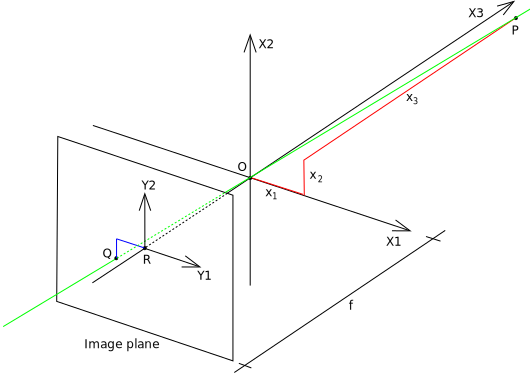
\includegraphics[width=0.7\textwidth]{pinhole3d}
}{fig:pinhole3d}{
	Pinhole camera geometry.
	Camera coordinate system origin at O, axis X3 points towards the optical axis, Y1 and Y2 point to image plane axes and R is the principal point, at the image center.
	The point P projects to Q, as well as everything else on the line joining them.
	The image plane is f units away from camera origin; f is called the focal length.
}
% FIXME z left handed?

Light rays travel through the pinhole camera's aperture to the image plane that is $f$ units behind the aperture, while the camera origin is set to the aperture.
The pinhole model (or, perspective projection) states that the world point $(x, y, z)$ is projected to the 2D image plane at $(u, v)$:

\begin{equation}
\begin{pmatrix}
u \\ v
\end{pmatrix}
=
-\frac{f}{z} \begin{pmatrix}
x \\ y
\end{pmatrix}
\end{equation}

The result can be derived from similar triangles with a common vertex at the aperture; figure \ref{fig:pinhole3d}.

Sometimes the sign is inverted, which results in a plane on the other side of the origin where the actual point lies, where the image is not rotated; this can be more convenient to analyse.
Physically, the projected point in a camera is behind the aperture, on the sensor.
\cite{hartley03multiview}

%Setting the camera to origin, the mapping is given with a camera matrix as
%
%\begin{equation}
%\begin{pmatrix}
%u \\ v \\ 1
%\end{pmatrix}
%=
%\begin{pmatrix}
%xf/z \\ yf/z \\ 1
%\end{pmatrix}
%\sim
%\begin{pmatrix}
%x \\ y \\ z/f
%\end{pmatrix}
%\sim
%\begin{pmatrix} \label{eq:cmat}
%	1 & 0 & 0 & 0 \\
%	0 & 1 & 0 & 0 \\
%	0 & 0 & 1/f & 0
%\end{pmatrix}
%\begin{pmatrix}
%x \\ y \\ z \\ 1
%\end{pmatrix}
%\end{equation}

The camera position and rotation in a global coordinate frame are encoded in a matrix transformation, so that the point $(x,y,z)$ in global coordinate frame is first transformed from a global coordinates to a camera-centered frame.
% Matrices, homogeneous coordinates.

% projective element, "~" up to scale equality definition

In computer graphics and vision, points and directions are usually described in \emph{homogeneous coordinates}.
Homogeneous coordinates add an extra dimension to the interpretation of coordinates, and each point becomes a line that crosses the origin in a dimension one higher than the original.
In addition, several vector operations become more convenient to manipulate; for example, 3D translation is embedded in 4D matrices with homogeneous coordinates. \cite{hartley03multiview,heyden2005multiple}
%Translation, perspective projection, rotation, and other operations are conveniently described as matrix transformations by using an additional dimension for points: $(x, y, z, 1)$.
The space is scale-invariant; all points $(xw, yw, zw, w)$ map to the same 3D point $(x, y, z)$.
\cite{dubrofsky2009homography,hartley03multiview}

%Homography definition (mapping of points and lines in $P^2$)

The imaging process essentially captures a projection to a flat two-dimensional plane of the camera's view.
When comparing points between different cameras that view the same scene, the cameras' relative positions and rotations must be known.
One of the cameras is often conveniently chosen as the origin of a global coordinate frame, so that its extrinsic parameters become unity transforms (programming libraries may assume this, see e.g. \cite{opencv}).
Each three-dimensional point in the world is transformed to the small sensor inside the camera, which is then digitized to a discrete two-dimensional grid of pixels, with different coordinate units.

%Figure \ref{fig:TODO} illustrates this transformation chain, which is encoded as the following equations, given a homogeneous point (4-dimensional vector) $X$ representing a 3D location described in physical (e.g. metric) coordinates:

The transformation chain is encoded as follows in eq. \ref{eq:projxform}, given a homogeneous point (4-dimensional vector) $X$ representing a 3D location described in physical (e.g. metric) coordinates:

\begin{align} \label{eq:projxform} \begin{split}
	x
	&= M_i X_s\\
	&= M_i M_p T R X\\
	&= M T R X\\
	&= P X\\
\end{split} \end{align}

$x$ is a 2d pixel in a discrete image, $X_s$ exists on the sensor.
$R$, $T$ encode the camera rotation and translation (extrinsics);
$M_p$ projects the world coordinates to the camera sensor - still in world coordinates, and finally the affine $M_i$ transforms the points from the sensor to pixel coordinates on the digital discretized image.
The transformation pipeline is depicted in figure \ref{fig:projxformworld}.

\simplegfx{p}{1.0\textwidth}{projxformworld}{
	Transformations in a projection matrix pipeline.
	FIXME: draft image
}


The whole projection $P = M_i M_p T R$ can be used as-is without decomposing it to separate matrices, unless the individual parameters are needed.
The matrices $M_i$ and $M_p$ are usually not decomposed but presented as a whole intrinsic matrix.
As the chain consists of several matrices, some of them are defined only up to scale; the coordinate systems' units can be chosen freely.
Software packages usually do not decompose the chain, because it is not needed and unique parameters cannot be found because of scaling.

%The external camera parameters are called the extrinsics: camera coordinate system position and rotation (heading) in the global space.
%Camera position sits at the projection center blah.

The internal parameters, intrinsics, encode how the image is formed on the sensor: they consist of focal length $f$, pixel size ($m_x$ by $m_y$) and principal point $(u_0, v_0)$:
% FIXME 3x3 3x4 4x4
\begin{equation}
	M =
	\begin{pmatrix}
		m_x & \gamma & u_0\\
		0   &    m_y & v_0\\
		0   &        0 & 1
	\end{pmatrix}
\cdot
	\begin{pmatrix}
		f & 0 & 0\\
		0 & f & 0\\
		0 & 0 & 1
	\end{pmatrix}
	=
	\begin{pmatrix}
		\alpha_x & \gamma   & u_0\\
		0        & \alpha_y & v_0\\
		0        & 0        & 1
	\end{pmatrix}
\end{equation}

For simplicity, it is often denoted $\alpha_x = m_x f$, $\alpha_y = m_y f$.
$R = (u_0, v_0)$ is the image center (or principal point).
The parameters can also be presented separately without the matrix notation.
For square pixels, $m_x = m_y$, and for a non-skewed (rectangular) sensor, $\gamma = 0$, which is often the case. \cite{hartley03multiview,szeliski10vision,heyden2005multiple}

%Le image. Horizontal planar triangle, lines between camera origins etc. lecture11.pdf.

% }}} coord systems and transforms

\subsection{Camera calibration} % {{{

\emph{Calibrating} a camera means \emph{measuring} its intrinsics and extrinsics in order to map its data to a known coordinate frame.
Reconstruction algorithms relate points between images to recover depth; the relations are specified via camera parameters.
Calibration is not necessarily a manual step before scanning;
self-calibration and structure from motion techniques can recover camera calibration from a static scene automatically. \cite{pollefeys1999hand,hartley03multiview}

It is sometimes convenient to store intrinsics and extrinsics separately if the intrinsic matrix is constant for several pictures, for example;
the intrinsics can then be calibrated beforehand only once.
For a camera rig that does not change, whole intrinsic and extrinsic calibration can be retrieved beforehand and applied on further scanned datasets for direct reconstruction.

Manual calibration is done with a known pattern, such as a planar checkerboard pattern \cite{chuang2002performance,zhang2000flexible} or manually selected point pairs.
A known pattern is fast to detect and results in correct physical units when the physical pattern size is given.
The checkerboard calibration step is often programmed to measure optical distortion at the same time. \cite{opencv,camcalmatlab}

A single image of a three-dimensional calibration object is also sufficient for single-camera calibration. \cite{jokukirjoist}

One way for calculating the calibration is direct linear transform (DLT):
the whole matrix $P$ is solved from $x_i = PX_i$ by constructing a system of equations from the projections of some known points $i$, and minimizing an error metric, as the case is usually overconditioned. \cite{hartley03multiview}

A video-based method has been proposed by Svoboda for self-calibration.
The method uses a number of synchronized frames and a laser pointer in a dark calibration volume to find corresponding points, not requiring any precise objects. \cite{svoboda2005convenient}

Structure from motion recovers full calibration for a larger amount of cameras with given matching point pairs, with no special requirements on the subject.
It can be used to calibrate an arbitrarily large unknown set of cameras automatically.
It is described further in section \ref{sec:sfm}.

%Projective calibration only is too general, as it leaves out some assumptions that can be done about a physical world, such as relative angles and sizes; metric calibration something something. \cite{zisserman1995metric}.

%Methods that dig the matrix out of a single image have certain restrictions, and won't work if e.g. seven points lie on the same plane [longuet-higgins etc.]

%many single planar chessboard pics vs. a single image of an accurate 3d model.
%Single three-dimensional calibration object is also sufficient blbl

%cv::stereocalibrate, cv::calibratecamera
%TODO Figure: show extrinsic in matlab cam calibs, nice pics (both cam and world centered)

% }}} camera calibration

\subsection{Preprocessing/normalization} % {{{

(to be moved)

%The scale of values in the equations above affects the precision [hartley, in defense of .., h,ziss]. 
The scale of values affects the numeric precision \cite{hartley1997defense,hartley03multiview}.
A similarity transform is used to modify the values to a more consistent range.
Centroid is moved to image center, and the coordinate axes are scaled.

%Translate centroid to the origin, scale so that average becomes sqrt 2.

Histogram and brightness equalization is done if image brightnesses vary for more effective point matching.
A well controlled stereo rig does not need color correction if the lighting is even enough.

% }}}

\subsection{Calibrated stereo vision} % {{{

Given two or more views of a same scene, depth for a point can be extracted by comparing the positions of the point in different views.
Whole-picture depth extraction results in a depth map imaged from a single view, giving a depth value for each pixel in a picture, resulting in a set of three-dimensional points seen by that view.
The resulting stereo vision consists of many steps.
In order to compare the point positions in two images, given a point in one image, its matching pair must be found on the other.
In the following section, this search problem in finding corresponding pixels, mapping them so that they can be compared, and the comparison that results a depth value are formalized.

% }}}

\subsubsection{Binocular disparity} \label{sec:binocular} % {{{

%Essential, fundamental matrices. Correspondence problem. Rectification, undistortion. Epipolar geometry.

\simplefig{h!}{
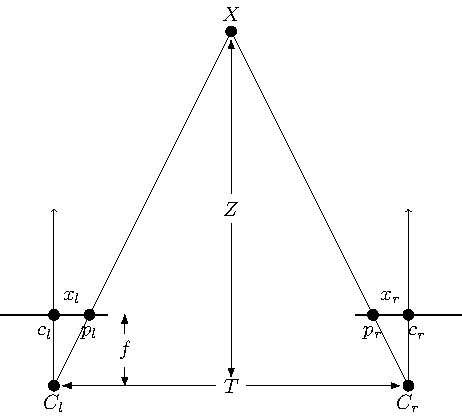
\includegraphics{simplestereo}
}{fig:simplestereo}{
	A very simple stereo setup, pictured from above.
	The image planes (thick lines) are actually imaginary, as a real film in a camera would exist behind the principal point and project the image as rotated around principal axis, as described earlier in \ref{sec:imaging}.
	The coordinates are given in units of the world coordinate system, common with the camera origins.
	The symbols $C$ are the camera origins ($T$ units between each other); $c$ the principal points; $x$ the image plane coordinates of $p$ w.r.t.~the principal points; and $f$ is the focal length.
	The unknown is $Z$, i.e.\ depth of point $X$.
}
% this figure would need to be bigger and have also the back side planes (sensors) as opposed to the (normalized?) image planes (at f=1?)

%Next, the setup of binocular stereo vision is described. Common stereo vision rigs use the simplest possible case: two identical cameras with a fixed distance, both oriented to the same direction, parallel to the line connecting them, as in figure \ref{fig:simplestereo}.

%Assuming known calibration with identical cameras (same focal length and sensor) in a setup described above, visualized in figure \ref{fig:simplestereo}, points can be triangulated as follows:
Assuming a planar setup with identical cameras (same focal length and sensor) facing in the same direction as visualized in figure \ref{fig:simplestereo}, points can be triangulated as follows:

From similar triangles with a common vertex at $X$, we get (note that $x_r < 0$ as it's to the left, towards to the negative axis, from the corresponding plane's origin):

\begin{align} \label{eq:triangulation} \begin{split}
	\frac{Z}{T} &= \frac{Z-f}{T - x_l + x_r} \\
	&= \frac{Z-f}{T - d}\\
	ZT - Zd &= ZT - fT\\
	Z &= \frac{fT}{d}
\end{split} \end{align}

The disparity $d$ is the difference of the points in their image planes, $d = x_r - x_l$.
%If the image planes would be fixed as being physically correct, in the back side of the camera origins, the focal length should be negated to keep the correct interpretation and sign because the projected physical image is mirrored in both axes.
%Image processing between the sensor and a picture file usually inverts this.
As the equation \ref{eq:triangulation} shows, depth is inversely proportional to pixel disparity in the images.
To map the depth to correct units, only focal length $f$ and the baseline $T$ are needed additionally; when using pixel coordinates instead of physical in $d$, also the pixel size should be taken into account in scaling $x_l$ and $x_r$.
All of these are encoded in the camera parameters: the pixel size is part of the intrinsics, and the baseline is encoded in extrinsics.
Algorithms such as those in OpenCV \cite{opencv} can compute depth from disparity images based on the difference between each pixel.
The disparty image is a difference of each pixel value, which needs a search for each pixel;
this is discussed in the following.

% }}} binocular disparity

\subsubsection{Epipolar geometry} % {{{

\simplefig{h!}{
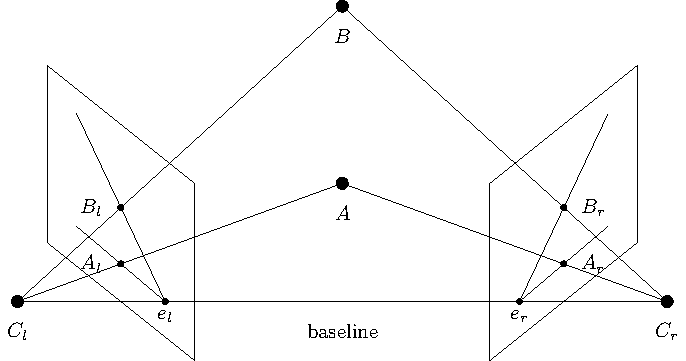
\includegraphics{epigeom}
}{fig:epigeom}
{Two camera views on same scene.
World points $A$, $B$ project to planes of different views imaged from $C_l$ and $C_r$ on the left ($A_l$ and $B_l$), and to the right ($A_r$, $B_r$).
The actual images cover some area of the total projection plane, and the epipolar point may or may not lie visible in the image.
When $A_l$ is known, its corresponding point $A_r$ (not initially known in practice) is found on the epipolar line joining $e_r$ and $A_r$ in the right image.
All epipolar lines in a view join in the same point ($e_l$ and $e_r$).}

% TODO: small algorithm for pairwise windowed point matching on the line (hox! and link to point matching section maybe)

In stereo vision, the same scene of interest is seen by two or more cameras at the same time.
The cameras are rarely aligned perfectly as in the disparity setup described above, however.
\emph{Epipolar geometry} encodes the relations between arbitrarily positioned cameras in a standard way so that coordinates of a 3D point seen in several images can be calculated with similar triangulation.

As seen in fig. \ref{fig:epigeom}, a point seen by camera $C_l$ at 3D point A could be anywhere on the line between $C_l$'s origin and A, because a certain line passing through the principal point always projects to a point.
This line is seen as a single point $A_l$.
From another viewpoint in camera $C_r$, this line equals to some line on the right image plane.
The matching point must be on that line.
The inverse applies for any point on $C_r$ and a line on $C_l$.
These special lines on the image planes are called \emph{epipolar lines}, and they all coincide at a special point called \emph{epipole}, $e_l$ and $e_r$.
For example, the line from $C_l$ to $A$ projects to the line from $e_r$ and $A_r$ on the right plane, and likewise, the line from $C_l$ to $B$ projects to the line from $e_r$ and $B_r$, which can be easily seen from the triangles in the figure.

% FIXME:
\emph{Essential matrix} encodes how the camera poses differ, to match one image's point in another.
When $A_l$, $A_r$ encode the points in figure \ref{fig:epigeom} by the corresponding camera coordinates, and the baseline difference is a vector from $C_l$ to $C_r$, it holds that $(A_l-C_l) \cdot (C_r - C_l) \times (A_r-C_r) = 0$, as all the vectors are coplanar; the cross product yields a normal to the plane, which is perpendicular to all the vectors, thus the dot product equals 0.
\cite{hartley03multiview}
Essential matrix $E$ is a matrix form of this relation; it includes the relative rotation and translation of the two cameras:

\begin{equation} \label{eq:essential}
	A_l E A_r = 0
\end{equation}

%\begin{align*} \label{eq:essential}
%	%A_r &= R (A_l - t) \\
%	%A_r^T R T A_l &= 0 \\
%	%A_r^T E A_l &= 0
%	A_l \cdot t \times A_r = 0\\
%	A_l \cdot t \times R A_r = 0\\
%	A_l^T T
%\end{align*}

%where $T$ is the cross-product form of $t$ encoded in a matrix form as below. The essential matrix is obtained as $E = R T$.
%
%Le image. lecture11.pdf. O->p dot (O->O' cross O'->p') = 0
%
%Cross product expressed in a skew-symmetric matrix form is
%\begin{equation}
%\vec a \times \vec b =
%\begin{pmatrix}
%	 0   & -a_z &  a_y\\
%	 a_z &  0   & -a_x\\
%	-a_y &  a_x & 0
%\end{pmatrix}
%\begin{pmatrix}
%	b_x\\b_y\\b_z
%\end{pmatrix}
%= \vec c
%\end{equation}

\emph{Fundamental matrix} is a similar object; it also relates the corresponding points in stereo images.
It has the same meaning as the essential matrix, but it works in the pixel coordinates of the cameras, which are obtained after the projective transform that takes the intrinsics into account; that is, it encodes also intrinsic parameters.
%Inverting the matrix $M_i$ (section \ref{sec:coord}) in sensor-to-pixel coordinate transform and using it on pixel coordinates, world coordinates seen on the camera sensor can be obtained. % FIXME equations

Given pixel coordinates $a_l$ and $a_r$ that match the points $A_l$ and $A_r$ as seen from cameras $C_l$ and $C_r$, respectively, the fundamental matrix $F$ is given as:

\begin{equation} \label{eq:fundamental}
	a_l F a_r = 0
\end{equation}


%\[
%\hat pAl = M_p A_l\\
%\hat A_r = M_p A_r
%\]
%
%and using it on pixel coordinates, the world coords can be obtained, plugging in to the equation \ref{eq:essential}
%
%\[
%A_r^T E A_l = 0\\
%(M_p^-1 \hat A_r)^T E (M_p^-1 \hat A_l) = 0\\
%\hat A_r^T M_p^-T E M_p^-1 A_l = 0\\
%\hat A_r^T F \hat A_l = 0
%\]
%
%the fundamental matrix
%
%\[
%F = M_p^-T E M_p^-1 = M_p^-T R T M_p^-1
%\]

The fundamental matrix relates directly the pixels and epipolar lines, and as such it is useful in image processing where the images are described as pixels in a raster image rather than physical coordinates.

%Le image above and lecture11.pdf. O->p dot (O->O' cross O'->p') = 0

%Cross product expressed in a skew-symmetric matrix form is
%\begin{equation}
%\vec a \times \vec b =
%\begin{pmatrix}
%	 0   & -a_z &  a_y\\
%	 a_z &  0   & -a_x\\
%	-a_y &  a_x & 0
%\end{pmatrix}
%\begin{pmatrix}
%	b_x\\b_y\\b_z
%\end{pmatrix}
%= \vec c
%\end{equation}
%
%Epipole can be interpreted as the location of another camera as seen by other camera, as seen in the picture.

%Now, given its position in the image plane of camera $C_l$ and the fundamental matrix $F$, finding the corresponding point in camera $C_r$'s image plane is seen as solving eq. \ref{eq:fundamental} for $a_r$.

The essential and fundamental matrices can be seen as a more general configuration of the triangulation in fig. \ref{fig:simplestereo} and eq. \ref{eq:triangulation}.
Once the points are found by solving \ref{eq:fundamental}, the depth can be obtained.

% cite longuet-higgins 1981, the books too

% }}} epipolar geometry

\subsubsection{Features and point matching} % {{{

%salient geometric features for matching

Previously, basics for reconstructing a three-dimensional location for a point pair were introduced, assuming known positions for the same point in different images.
To reconstruct a whole scene from a full image, all pairwise points must be \emph{matched}, i.e.\ found that what pixel in one view represents the same object as one in other view.

Matching is often also called \emph{correspondence} searching:
Given a pixel in one image, what is the corresponding pixel in another image taken from the same scene?
Pixels correspond to each other if they represent the same physical point.
Matching pixels for the previously introduced methods are found in the image space by comparing the color neighborhood.

% FIXME: pairwise feature matching vs. windowed matching
% TODO some sift descriptor theory, angle histogram stuff

To describe the pixel's visual characteristics, its surrounding environment is encoded as a \emph{feature}, an easily recognizable property vector, \emph{feature descriptor} or \emph{feature vector}.
%When discussing about features, not every pixel's neighbourhoods are used; \emph{good} features are those that have strongly distinguishable properties, such as edges and corners.

Edges or corners are essentially high-frequency information in the image that can be interpreted as a 2D discrete function; thus, they can be detected by a discrete high-pass or band-pass filter, zeroing all but those pixels where a high difference is found. \cite{marr1980theory}
Many feature detector algorithms are based on edge detection. % CITE

Scale-invariant feature transform (SIFT) \cite{lowe1999object} is a well-known algorithm for local feature detection. A fast GPU implementation is also available \cite{changchang2007siftgpu}.  Invariance to scaling and rotation makes SIFT useful in describing features that can be matched between unaligned images. Other similar commonly used means are Speeded Up Robust Features (SURF) \cite{bay2006surf}, Harris corner detector \cite{harris1988combined}, and difference-of-gaussian-based (DoG) methods \cite{dog}.

Searching for well distinguished features in an image is called \emph{sparse} search.
A sparse set of feature matches is good for reconstructing initial calibration, as all the feature vectors can be matched together relatively quickly.
For finding a complete depth map of the whole image, a slower \emph{dense} search is performed, using the obtained calibration.
Dense matching runs through each pixel of the search space and tries to find a matching pixel from another image with e.g. template matching \cite{duda1973pattern}.
The surrounding pixel values themselves inside a \emph{window} centered at the searched pixel are compared in the search area.

From the coordinate differences in image space between the two images, a disparity map is built.
The disparities can then be directly transformed to depth values, yielding a point cloud.
Other more sophisticated algorithms too find dense matches but may not use a disparity map.

% }}}

\subsubsection{Image rectification} % {{{

% rectification pics

In order to triangulate a 3D point from two photographs, the location of the point in both the images must be known.
The dense correspondence search is not done with feature matching but comparing pixels directly instead.
Given a single pixel in one image, its corresponding pair would naively be searched by looking at every possible pixel in another.

Rectification is a process that simplifies this search problem by restricting the search to a single dimension using the epipolar lines.
Further, closeby points are only looked in a small window around the previous, not spanning the whole search space.

By virtually aligning the cameras such that their images are coplanar, the search only has to be performed on a line that is parallel to the line connecting the camera centers.
Rectification can be done in multiple ways.
Planer rectification projects the images on a common plane and rotates them such that corresponding lines are axis-aligned (horizontal or vertical) in both images. \cite{hartley03multiview}
In figure \ref{fig:rectif}, two cameras are situated at arbitrary positions, looking at different directions, and their view images are projected on a common plane, where they show up as trapezoids.
In practice, a new image can be created that contains the old trapezoidal image, or the search can be performed in the original image in the direction of the epipolar line.

\simplegfx{h}{0.6\textwidth}{rectif}{
	In planar image rectification, two images are twisted so that the epipolar lines (drawn in red) become parallel.
}


%Rectified images are twisted so that todo todo, see figure \ref{fig:rectification} compare to epipolar geometry image, epipolar lines become parallel in the rectified images
% LOL TODO guido gerig image rectification (stereo) slides

% }}} correspondence and rectification

\subsubsection{Multi-view stereo} % {{{

(highly incomplete section)

% nelliportaali:pikahaku multiview stereo reconstruction
%graph cuts
%\cite{jancosek2011multi}
%\cite{chang2011gpu}
%(this section needs expansion and pictures)
% if no information about camera parameters is available, pairwise checks between the images may become expensive. \cite{wu2013towards}
%evaluations in \cite{goesele2007multi}
% se zephyrpapru jossa algossa per kamera depth ja merge

% intro

\emph{Multi-view stereo} (MVS) is stereo vision using more than two cameras.
In the literature, MVS refers to both the big picture of a whole reconstruction pipeline using several pictures, and just the dense reconstruction after system calibration has been done.
Reconstruction using a large set of cameras has two distinct major ways to perform:
One way is to extend the two-view geometry theory further to many cameras, recovering the whole subject at once using many views simultaneously.
Other, also commonly used method is to arrange the cameras in binocular pairs, reconstruct each pair separately to obtain a depth map from each pairwise view, and finally merge the resulting points to a single set. \cite{bradley2010high}

% epipolar in N

The case of more cameras than a single pair uses the same epipolar geometry principles, extended in several ways.
More cameras bring more dimensions, complications and also restrictions that can be utilized.
In three-view geometry, for example, the fundamental matrix becomes three-dimensional, the trifocal tensor, relating all three cameras to the others. \cite{hartley03multiview}

Some suggest to find a set of initial features and expand them to nearby pixels. \cite{furukawa2010accurate, regiongrowingtodo}

Multiple baseline stereo is a simple special case for many cameras. When all the cameras lie on the same baseline, calibration is easier and points seen by all cameras can be selected simply by using a minimized sum of errors. \cite{okutomi1993multiple}

An incremental algorithm linear-time in number of the cameras has been suggested for SfM for large-scale reconstructions. \cite{wu2013towards}
A specialized scanning rig in this work is not considered large-scale.
Large-scale refers to hundreds or even thousands of images of a huge geometry, such as an outdoor building or terrain.
A state-of-the-art patch-based reconstruction combined clustering to split large-scale datasets produces dense, oriented point sets \cite{furukawa2012patch,furukawa2010accurate}

Toldo et al. suggests to build a depth map individually per each view with approximated normals, and to combine the points to a mesh with Poisson surface reconstruction. \cite{toldo2013accurate,toldo2013towards}

% }}} multi-view stereo

\subsection{Structure from motion} \label{sec:sfm} % {{{


The \emph{structure from motion (SfM)} problem, also called structure and motion, uses the scene feature matches between different views to determine both the scene structure and the camera motion between the views.
\cite{snavely2006photo,fitzgibbon1998automatic} 
The camera does not have to physically move; the method can be used for multi-camera reconstruction with a static rig.
Before SfM, the images should have been rectified and features matched; the algorithm works on point locations instead of input images.
While SfM retrieves the scene structure and camera parameters, a dense reconstruction usually follows it as only a fraction of the points in the images need to be considered.

SfM begins with two reference views that are used to retrieve an initial reconstruction, and extends each new view into the set iteratively.
Lastly, a \emph{bundle adjustment} method is used to globally optimize the scene parameters. \ref{triggs2000bundle}
The relation between the views need not be previously calibrated; the process determines camera poses.
In fact, many reconstruction applications use structure from motion as an initial step to determine calibration and proceed then to dense reconstruction.

The initial stage builds a reference frame and structure for the selected features (points) in two cameras.
% pollefeys tutorial builds the frame using the epipolar geometry, determined as previously in section \ref{sec:epipolar}.
The structure is determined with triangulation as in section \ref{sec:binocular}.
In practice, perfect reconstruction cannot be achieved due to noise, and the points are found by minimizing a reprojection error to the extent of a specified threshold limit.

After a coordinate frame is built as a basis using two views, the next camera views are iteratively added to obtain an initial estimate of the camera poses and the selected scene feature positions.
Scene features can be matched between only last few views if the camera motion is known to be continuous;
the matches can also be done between all possible image pairs, which is feasible if there is lots of overlap.

As a last step, bundle adjustment globally optimizes the bundles of light rays from the scene to all cameras.
Several algorithms and implementations are available, while the basic idea and the underlying problem is the same:
a cost function is used to optimize jointly all camera parameter estimates such that the reprojection errors are minimized through all views.
Pollefeys \cite{tutorial} gives the following formula to minimize:

\begin{equation}
	\text{min}_{P_k, X_i} \sum_{k=1}^m \sum_{i=1}^n D(x_{ki}, P_k X_i)^2
\end{equation}

when the goal is to find the projection matrices $P_k$ and the 3D points $X_i$ for all views $k$ and points $i$, where $D(a,b)$ is the Euclidean distance and $x_i$ the known, fixed matching 2D image feature positions for each unknown 3D point $X_i$.
In practice, this nonlinear optimization problem is approached in iterative means.

According to \cite{wu2013towards}, bundle adjustment should be performed using a Levenberg-Marquardt or Preconditioned Conjugate Gradient method.

Beardsley et al. use an iterative extended kalman filter \cite{beardsley1997sequential}
% XXX others?

% }}}

\subsection{Error metrics} % {{{

The quality of the reconstruction is measured by reprojecting the 3D points back to the cameras with the estimated parameters, and calculating the distance between the projected and the matching original point, the \emph{reprojection error}. \cite{hartley03multiview}

Furthermore, if the scene structure is known beforehand (e.g.\ as a calibration object, whose physical properties are measured), the resulting quality of the structure can be compared to ground truth.
Ground truth data can also be obtained with a real 3D scanner, such as a laser ranging device. % david

%Noise in subpixel-accurate match detection and (TODO survey errors, that one .doc) affects each reconstructed depth.
In addition, uncertainty in depth depends more heavily on the pixel errors (i.e.\ disparity) if the baseline is short, depicted in figure \ref{fig:disparityerror}. % TODO image, recent in the paper notebook

Bundle adjustment optimizes uncertainty in camera poses and projection matrices together.

When sparse feature matches are searched for matching picture points in different views, a number of features are first generated for each picture, and the matches are tested against picture pairs.
False positive matches should be filtered out; common way to handle feature errors is Random Sample Consensus (RANSAC).
Random subsets of the sample space is iterated, and samples that do not fit well to a model that is constructed for a smaller set are ignored.
The iteration that matches most samples is selected. \cite{hartley03multiview}

%Detail calculation (error on surface ~= avg reprojection error?) compute millimetres

Practically, the camera sensor size and focal length in physical units (millimetres) are known, making conversion from pixel units to millimetres possible.
Units originating from reconstruction of raster images can be simply scaled to millimetre units, resulting in more intuitive error interpretation.

%Compare to algebraic, geometric etc.

%Mesoscopic level shape reconstruction

% }}}

\subsection{Surface fitting} % {{{

A multi-view reconstruction results in a set of three-dimensional points, with no \emph{connectivity information}, i.e.\ interpretation of \emph{surfaces}.
In reality, all the pixels are projections of nearby surfaces, and a more natural and standard representation can be obtained by fitting a surface on the points.
Surfaces in computer graphics are described as collections of small patches with a polygon outline, often just triangles.
When rendering the points on a computer screen, pixels between them are interpolated to contain all color information available in the source photographs.

% }}} surface fitting

\subsubsection{Data structures} % {{{

\simplefig{h}{%
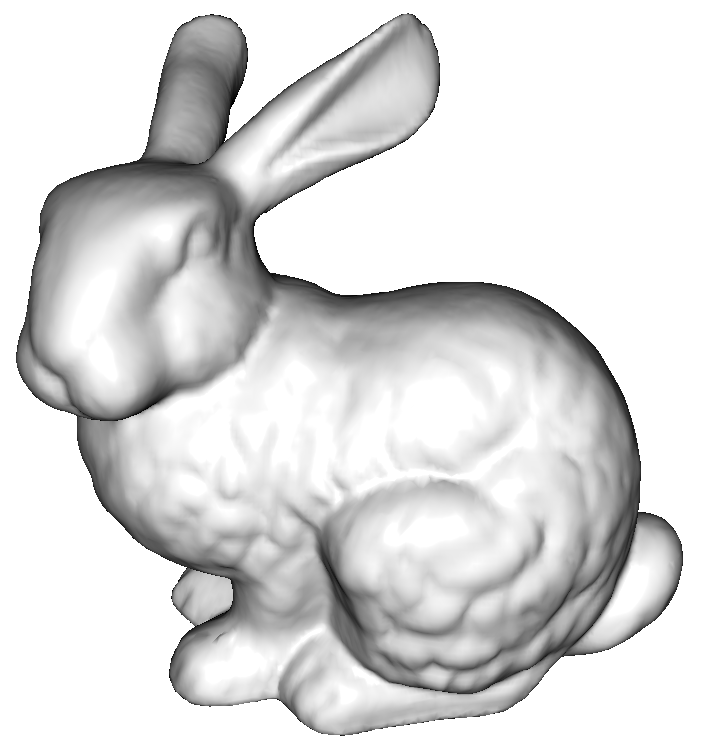
\includegraphics[width=0.3\textwidth]{bunny}
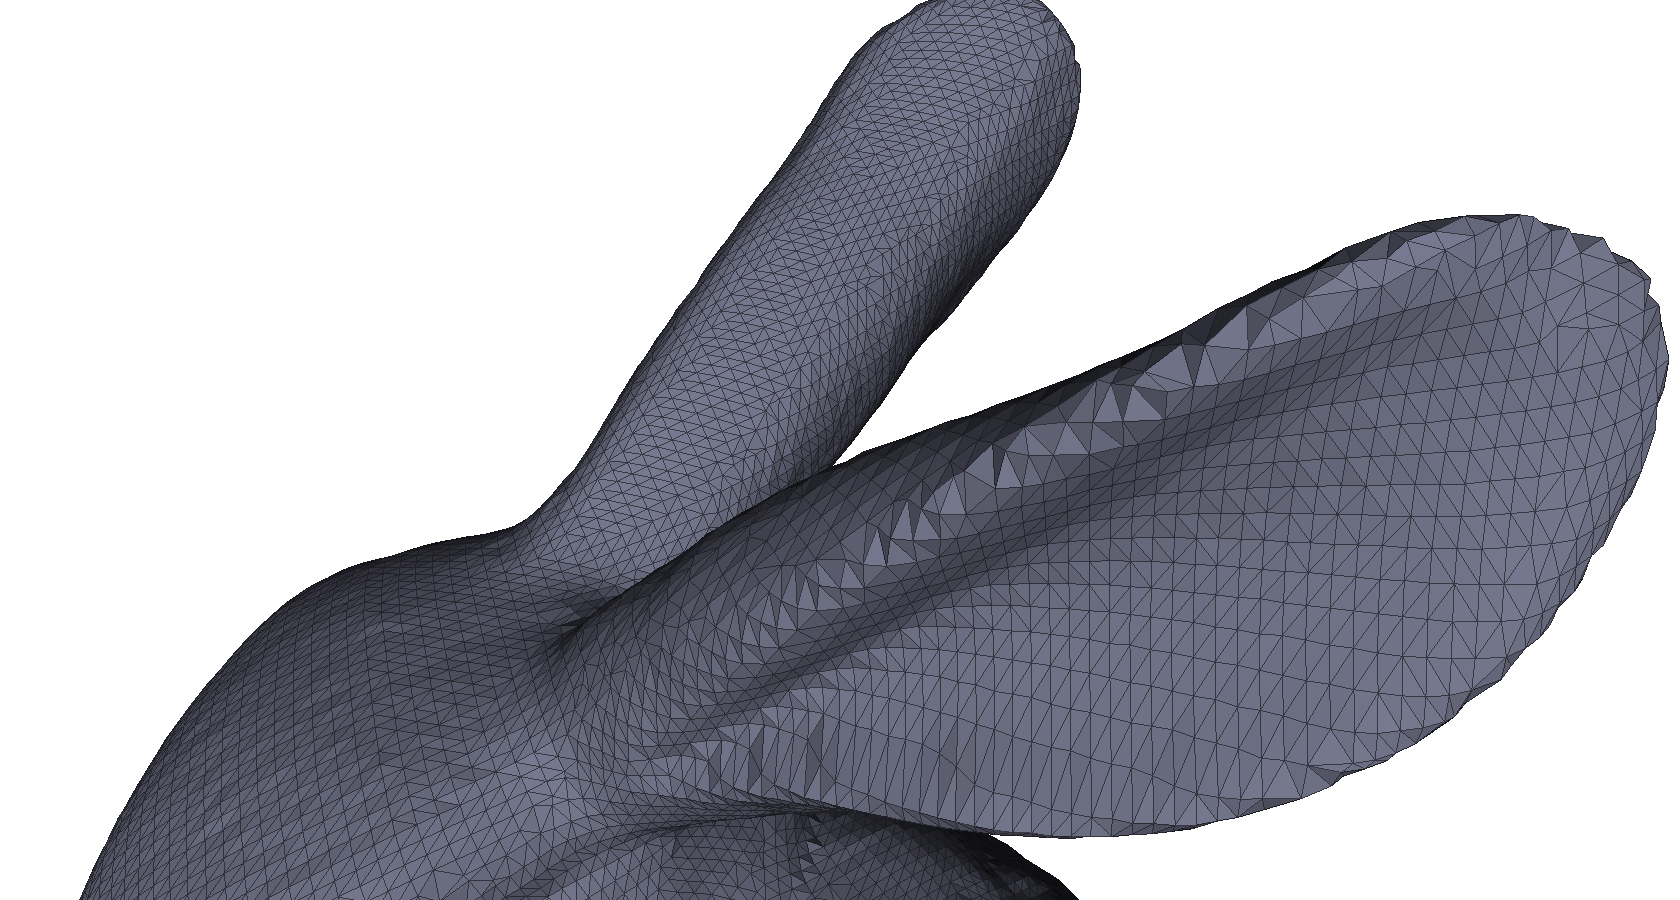
\includegraphics[width=0.6\textwidth]{bunnyear}
}{fig:stanfordbunny}{
	Stanford Bunny, a standard 3D test model by The Stanford 3D Scanning Repository, Stanford Computer Graphics Laboratory, scanned with a laser ranger.
	On the left: the whole model, shaded with a simple Phong model.
	On the right: a closeup of the left ear, showing the borders of the faces as black lines connecting the vertices.
}

% http://en.wikipedia.org/wiki/File:Mesh_overview.svg

(Should some of the main terms be defined in the beginning of the whole thesis? Probably...)

A \emph{(polygon) mesh}, a data structure often used to describe 3D models, consists generally of \emph{vertices} connected by \emph{edges}, forming \emph{faces} of objects.
The meshes often consist of triangles, which is the simplest possible polygon.
Polygon meshes have a \emph{topology}; the connectivity information of vertices on a surface, describing neighbours of each point.
Surface \emph{normals} describe the orientation of the polygon patches.
Figure \ref{fig:stanfordbunny} depicts the vertex structure of a 3D model.

A \emph{point cloud} is a loose term to describe a disorganized set of 3D points with no topology information; that is, a cloud consists only of a list of vertices, with possibly some attributes such as color or normal.
Point cloud is a natural output format for 3D reconstruction, as each point in the cloud maps to some pixel in a source image.
The images and the depth information of the 3D points are not enough for surface information, which is covered next.

% }}} data structures

\subsubsection{Geometry} % {{{

Assuming that the recovered 3D point cloud represents the surface of an object, the next step of interest is to recover the surface topology from the point cloud.
The point cloud is all geometric information that is available, but the images probably consist of more pixels than the number of points in the point cloud.
To work with the generated model and to render it properly with colors, it is imporant to recover the topology information.

A popular method for surface reconstruction from a point set is \emph{marching cubes}. \cite{lorensen1987marching}
The algorithm builds triangles in a divide-and-conquer approach based on whether points are inside or outside a cube in a grid.
A number of improvements have been proposed that utilize marching cubes as a final step.
The method of choice is currently \emph{poisson surface reconstruction}. \cite{kazhdan2006poisson,kazhdan2013screened}

Before fitting a surface on the points, the point data set should be processed either manually or automatically to remove outliers.
The surrounding scene might contain geometry that is not part of the scanned object, which will affect badly the surface fitting algorithm.
Specular highlights and other artifacts on the surface may also introduce outliers.
Manual work is a simple way to delete the points that are not part of the actual object, but also automatic methods exist if manually filtering the subject would be repetitive, e.g.\ many expressions on a human face.

% assuming X on the geometry to fit a model

% }}} geometry

\subsubsection{Texture reprojection} % {{{

When a polygon mesh is available, it should be rendered in color, including the areas between the original points.
The de facto method in computer graphics is to uses \emph{texture mapping} to color pixels in between the vertices, when the number of vertices is less than the number of pixels on the screen.
A \emph{texture coordinate} is set for each vertex in the mesh to \emph{map} a smaller image from the texture on to the particular polygon. \cite{heckbert1986survey}

Building the texture is done in a similar way of rendering the image on a screen or capturing a scene with a camera:
The reconstructed mesh surface is projected on the raster images, registering the image coordinates on each vertex. \cite[p. 610]{szeliski10vision} \cite[p. 98]{heyden2005multiple}
When the mesh is viewed from another viewpoint, the pre-projected texture data is used again.
Great accuracy can be acheived if a MVS structure is combined with a laser scan, by registering the point clouds generated by both together, using the laser scan as geometry and registered camera poses to project textures. \cite{liu2006multiview}
% (XXX read meshlab src, references?)
% parameterization + texturing from registered rasters

When several cameras see the same view, the correct texture must be chosen on each vertex.
The selection can be taken based on e.g. the image with highest detail or best brightness.

%use the registered raster projections to find out best textures and build uv coordinates
% TODO
\simplegfx{h}{0.6\textwidth}{texreproj}{
	Texture mapping a triangle from a color image on a virtual image plane on a computer screen as $m_v$.
	The triangle geometry is mapped on the color images, or textures, of the real cameras as $m_i$, and the triangular patch between the image vertices is stretched on the rendered triangle.
	Image from \cite[p. 98]{heyden2005multiple}.
}


% }}} textures

%\subsection{Postprocessing} % {{{
%
%(how the stored geometry is different from the rendered one; mathematical models in fragment shaders to use the texture variations / normal maps etc.)
%
%Error removal; strip outliers that do not have nearby pairs; small disconnected islands.
%
%Postprocessing: remodel the mesh (face), see what it would look like.
%Refine parameters to get a similar output as in the photos (normal map etc.), backproject.
%Use colors and highpass them; assume uniform lighting and locally uniform texture color (bradley).
%(Simply a rendering technique, that level of detail in 3D structure might not be needed).
%%Still, structured light and/or shading assumptions [shape from single image cues/shading trucco+verri p.225] done too.
%
%(video: 3d topology different in each frame; most algos do just stills. simple to combine them to a pre-recorded mesh)
%
%Rendered facial animation: on bones and stuff.
%% }}}

\clearpage
\section{Motion capture} % {{{

\emph{Motion capture} (mocap, or mo-cap) is the practice of recording object movement over time.
A recorded subject can be e.g.\ a human that has a skeletal model, possibly encoding also some skin movement.
In computer animation, the movement data is encoded as positions of certain vertices at each recorded point in time, and often post-processed to be parameterized to e.g.\ joint angles.
\emph{Surface capture} is a related term referring to a similar motion recording but happening on a locally deforming surface instead of a globally moving skeleton.

% It is possible to assume locally smooth movements in most areas; thus, a more intelligent approach should be used than simply reconstructing a new mesh for each frame and using registration to just align them.
% By making certain assumptions on high-resolution texture, very detailed bump maps can be extracted, for example, by backprojecting the expected 3d mesh to textures and refining. [CITE]

% }}} mocap

\subsection{4D data capture} % {{{

The reconstruction field uses the term \emph{4D} in the context of time-varying 3D data.
Analogous to the case of traditional 2D video consisting of separate discrete frames of pixels, a sequence of dynamic 3D data is, in a simple case, individual ``frames'' of point clouds.

For a source data in the form of video files per camera, effectively a sequence of synchronized pictures, each set of frames can be considered a static geometry on which the reconstruction would be done.
A naive alignment to e.g. previous or first frame is possible to average out the object movement if only its local surface movement is of interest.
Still, reconstructing each frame group separately would not produce the same topology for the mesh, as each frame contains a different point cloud and is not connected to the previous reconstruction, unless some algorithm that takes this into account is used.

Possibilities to correct the lack of coherent geometric structure exist.
Common ways include fitting each frame of the mesh to another pre-recorded or pre-modeled mesh \cite{somewhere,remedysoftware?} and matching to the previous frame iteratively.
%Later usage may need only the tracked positions of specific locations on the surface to deform a mesh with bone guides.

% }}}

\subsection{Geometry tracking} % {{{

%Kalman
%Fiducials / AR
%perf of cloth anim capture

The dynamic reconstruction requires tracking of individual points or objects in order to usefully handle the moved subject.
Non-static human motion capture in video gaming or movies, where post-processing time is available, rely on manual work to perfect the quality.
In realtime applications, the full frame is typically not reconstructed again, but only selected keypoints that are tracked in 2D are triangulated, and a previously scanned model is deformed based on them.
%A realtime case would need to e.g.~automatically register each frame between the previous one to use the geometry's dynamic properties.

However, the simplest tracking method is to leave tracking out completely: depending on the application, tracking might not be needed if the work done on the three-dimensional data does not need e.g. topological coherence in the time domain, but recomputes its work on each new point cloud.

%Registration and tracking of point clouds or meshes is a large topic on its own; this section reviewes only some of the most common methods presented in the literature.
%Some work with the reconstructed 3D structure; others use the source images and do additional work.

In three dimensions, a template model is often scanned beforehand that is then morphed to match the target object to keep the topology (i.e.~vertex neighborhood connectivity) constant.
This technique adapts well to non-rigid deforming subjects. \cite{bojsen2012tracking,li2009robust}
Common method also for the entertainment industry is \emph{animation retargeting}: using a completely separate character, and deforming it on each frame based on the current state of the scanned object, fitting the model's vertices to the scanned set.
% siggraph14 doghead

% }}} geometry tracking

\subsection{2D surface tracking} % {{{

%* SIFT/SURF/Harris feature tracking, reproject
%* edgels (edge pixels)

In two dimensions, the dense reconstruction step can be skipped when using only features in image space, providing real-time performance. \cite{pilet2005real}
Assuming that a precise object stays in the imaged volume, features can be detected and mapped to a point on the 3D surface, and tracked locally with no full-image reconstruction, while the tracked object is assumed to keep the same topology as a previously scanned model.

%http://en.wikipedia.org/wiki/Facial_motion_capture the polar express, beowulf
%Facial animation does not necessarily even need multi-view stereo for tracking and driving a predesigned character \cite{chuang2002performance,deng2007computer}.

Classic motion capture uses special reflective markers that are tracked in 2D with infrared cameras.
Distinctive bright markers are easily thresholded from the background, tracked, and triangulated in real time.
Markerless surface capture detects image features that are then used as virtual markers, working in a similar way.
Matching textured objects is more computationally intensive, and needs high resolution cameras.

Markerless capture is important in scanning facial movement, because time-varying texture is significant in highly dynamic and detailed deformations, such as wrinkles from different facial expressions.
Practically, scanning a neutral and wrinkled static subject beforehand and morphing between their texture is easier.

Tracking is done by looking for the same feature as in a previous frame in the neighborhood where it was previously.
State-of-the-art 2D tracking methods include Kanade-Lucas-Tomasi (KLT) \cite{KLT}, Tracking-Learning-Detection (TLD) \cite{TLD}, and Consensus-based Matching and Tracking (CMT), all based on \emph{optical flow}.
\cite{horn1981determining,gibson1950perception,beauchemin1995computation}
Given source and destination images, optical flow is the apparent motion in the scene, given as a motion vector for each pixel.
Estimating the flow is based on the brightness constancy constraint: the intensity (i.e.\ color) of the source and destination pixels is the same.
Optical flow is also used in morphing frames between frames in a video to virtually synchronize the cameras to a common clock. \cite{thatbradleyone}
% The Matrix.

%By combining the movement tracking to a mesh whose dynamics are modeled physically, motion can be estimated from a single image. \cite{decarlo1996integration} % (not in the scope)

% }}} 2d tracking

\subsection{3D registration} % {{{

Aligning two meshes or point clouds together is called \emph{registration}.
Registration finds a rigid transformation from one object to another.
For a moving subject, the method can be used to find the object movement between the frames.
Registration is also used for combining different, overlapping parts of a subject generated from different viewpoints to one larger model.

The basic idea in registration is to fit two surfaces or point clouds together so that the shapes that they present become as close as possible to each other.
The practical method of choice is iterative closest point fitting (ICP).
ICP iteratively finds a rigid transformation that minimizes the distance between every point in one mesh and its closest match in the other.
When tracking the deformation of a surface, the point sets describe a different geometry and there will always be some error.

When ICP is used locally, it can be applied to non-rigid cases too. \cite{brown2007global}

%Also e.g. ransac for removing noise. \cite{zhao2005alignment}

% kalman?

% }}} registration
